% Koma-Script Report, verkleinerte Überschriftenstile, Linie unter der Kopfzeile
\documentclass[ 11pt
				,ngerman
				,headsepline
				,headings=small
				,numbers=noenddot %kein Punkt hinter letzter Gliederungsziffer Abschnitt 2.1 statt 2.1.
				,draft=false
				,BCOR=0mm %Wert für Bindekorrektur kann hier eingestellt werden
				,DIV=12
				,captions=tableheading
				,paper=a4
				,abstracton
                ]{scrreprt}

%%%%%%%%%%%%%%%%%%%%%%%%%%%%%%%%%%%%%%%%%%%%%%%%%%%%%%%%%%%%%%%%%%%%%%%%%%%%%%%
% Basispakete
%%%%%%%%%%%%%%%%%%%%%%%%%%%%%%%%%%%%%%%%%%%%%%%%%%%%%%%%%%%%%%%%%%%%%%%%%%%%%%%
\usepackage[utf8]{inputenc} 
\usepackage[ngerman]{babel} %Anpassungen an nicht-englische Sprachen
\usepackage{ifpdf} 
%%%%%%%%%%%%%%%%%%%%%%%%%%%%%%%%%%%%%%%%%%%%%%%%%%%%%%%%%%%%%%%%%%%%%%%%%%%%%%%
%%%%%%%%%%%Änderung durch T.C  
            
              
                
%%%%%%%%%%%%%%%%%%%%%%%%%%%%%%%%%%%%%%%%%%%%%%%%%%%%%%%%%%%%%%%%%%%%%%%%%%%%%%%
% Schriftarten, Schriftschnitte etc.
%%%%%%%%%%%%%%%%%%%%%%%%%%%%%%%%%%%%%%%%%%%%%%%%%%%%%%%%%%%%%%%%%%%%%%%%%%%%%%%
\usepackage{fourier} %PDF-kompatible Schriftfamilie "Utopia", Freierhältliches Look-alike: Heuristica
\makeatletter % Warnungen zu Schriftartersetzungen unterdrücken
  \let\@font@info\@gobble
  \let\@font@warning\@gobble
\makeatother

\usepackage[official]{eurosym} % Eurosymbol
\DeclareUnicodeCharacter{20AC}{\euro} % Standard-Euro-Symbol wird durch qualitativ hochwertiges Eurosymbol ersetzt

\renewcommand{\caplabelfont}{\bfseries} % Fettdruck für Abb. und Tab.

\usepackage{color}
\definecolor{ercred}{RGB}{229,48,39}

\usepackage{setspace} % Einstellen von Zeilenabständen
\onehalfspacing % Anderthalbzeiliger Satz

\setlength\parskip{\medskipamount} % Abstand zwischen zwei Absätzen
\setlength\parindent{0pt} % Keine Einrückung in der ersten Zeile eines Absatz

\AtBeginDocument{
  \renewcommand{\labelitemi}{\(\triangleright\)} %definiert die Art der Aufzählungszeichen
  \renewcommand{\labelitemii}{\(\bullet\)}}
%%%%%%%%%%%%%%%%%%%%%%%%%%%%%%%%%%%%%%%%%%%%%%%%%%%%%%%%%%%%%%%%%%%%%%%%%%%%%%%

%%%%%%%%%%%%%%%%%%%%%%%%%%%%%%%%%%%%%%%%%%%%%%%%%%%%%%%%%%%%%%%%%%%%%%%%%%%%%%%
% Layout der Seiten
%%%%%%%%%%%%%%%%%%%%%%%%%%%%%%%%%%%%%%%%%%%%%%%%%%%%%%%%%%%%%%%%%%%%%%%%%%%%%%%
\usepackage{fancyhdr} %Einstellung der Kopfzeile, Chaptermark auskommentieren wenn ein Stil one Kapitel gewählt wird (z.B. scrartcl)
\pagestyle{fancy} % Notwendig um die nächsten beiden Neudefinitionen vorzunehmen
\renewcommand{\sectionmark}[1]{\normalsize\markright{\thesection{} #1}{}}
\renewcommand{\chaptermark}[1]{\normalsize\markboth{#1}{}}
\interfootnotelinepenalty=10000 % Fußnoten nicht über zwei Seiten verteilen
%%%%%%%%%%%%%%%%%%%%%%%%%%%%%%%%%%%%%%%%%%%%%%%%%%%%%%%%%%%%%%%%%%%%%%%%%%%%%%%

%%%%%%%%%%%%%%%%%%%%%%%%%%%%%%%%%%%%%%%%%%%%%%%%%%%%%%%%%%%%%%%%%%%%%%%%%%%%%%%
% Tabellen
%%%%%%%%%%%%%%%%%%%%%%%%%%%%%%%%%%%%%%%%%%%%%%%%%%%%%%%%%%%%%%%%%%%%%%%%%%%%%%%
\usepackage{longtable}
\usepackage{multirow}
\usepackage{booktabs} % erzeugt besser aussehende Tabellen, horizontale Linien mit \toprule, \midrule, \bottomrule
\usepackage[point]{rccol} %Richtet Zahlen in Tabellen nach Dezimalkomma aus, im Output wird ein Dezimalpunkt verwendet
\usepackage{lscape}
%%%%%%%%%%%%%%%%%%%%%%%%%%%%%%%%%%%%%%%%%%%%%%%%%%%%%%%%%%%%%%%%%%%%%%%%%%%%%%%

%%%%%%%%%%%%%%%%%%%%%%%%%%%%%%%%%%%%%%%%%%%%%%%%%%%%%%%%%%%%%%%%%%%%%%%%%%%%%%%
% Abbildungen
%%%%%%%%%%%%%%%%%%%%%%%%%%%%%%%%%%%%%%%%%%%%%%%%%%%%%%%%%%%%%%%%%%%%%%%%%%%%%%%
\usepackage{subfigure}
\usepackage{float}

%%%%%%%%%%%%%%%%%%%%%%%%%%%%%%%%%%%%%%%%%%%%%%%%%%%%%%%%%%%%%%%%%%%%%%%%%%%%%%%

%%%%%%%%%%%%%%%%%%%%%%%%%%%%%%%%%%%%%%%%%%%%%%%%%%%%%%%%%%%%%%%%%%%%%%%%%%%%%%%
% Mathematik
%%%%%%%%%%%%%%%%%%%%%%%%%%%%%%%%%%%%%%%%%%%%%%%%%%%%%%%%%%%%%%%%%%%%%%%%%%%%%%%
\usepackage{amsmath}
\usepackage{amssymb}
\usepackage{array}
\usepackage[cdot,thickqspace,squaren,textstyle]{SIunits} % SI-Einheiten sind als Befehle verfügbar
%%%%%%%%%%%%%%%%%%%%%%%%%%%%%%%%%%%%%%%%%%%%%%%%%%%%%%%%%%%%%%%%%%%%%%%%%%%%%%%

%%%%%%%%%%%%%%%%%%%%%%%%%%%%%%%%%%%%%%%%%%%%%%%%%%%%%%%%%%%%%%%%%%%%%%%%%%%%%%%
% Referenzen und Zitate
%%%%%%%%%%%%%%%%%%%%%%%%%%%%%%%%%%%%%%%%%%%%%%%%%%%%%%%%%%%%%%%%%%%%%%%%%%%%%%%
\usepackage{varioref}
\usepackage[square]{natbib}
\usepackage{bibunits}
%%%%%%%%%%%%%%%%%%%%%%%%%%%%%%%%%%%%%%%%%%%%%%%%%%%%%%%%%%%%%%%%%%%%%%%%%%%%%%%


%%%%%%%%%%%%%%%%%%%%%%%%%%%%%%%%%%%%%%%%%%%%%%%%%%%%%%%%%%%%%%%%%%%%%%%%%%%%%%%
% PDF-Einstellungen
%%%%%%%%%%%%%%%%%%%%%%%%%%%%%%%%%%%%%%%%%%%%%%%%%%%%%%%%%%%%%%%%%%%%%%%%%%%%%%%
\ifpdf
	%we are running PDFLaTeX
	\usepackage[pdftex]{graphicx} 
	\pdfimageresolution=100
	\pdfminorversion=7
	\pdfcompresslevel=9
	\usepackage[pdftex,
		urlcolor=blue,
		linktocpage,
		colorlinks=true,
		linkcolor=black,
		citecolor=black,
		pdfview=FitH,
		pdfstartview=FitH,
		plainpages=false]{hyperref}
	\hypersetup{
		pdfauthor={Deine Name},
        pdftitle={Titel des Berichts},
        pdfsubject={},
        pdfkeywords={Mehrere aussagekräftige Schlagwörter},
        pdfproducer={LaTeX with hyperref},
        pdfcreator={pdflatex}}
    \usepackage[figure,figure*]{hypcap}
\else
	%DVI or PS output
	\usepackage{graphicx} 
\fi

%%%%%%%%%%%%%%%%%%%%%%%%%%%%%%%%%%%%%%%%%%%%%%%%%%%%%%%%%%%%%%%%%%%%%%%%%%%%%%%

\begin{document}
\pagestyle{empty}
\newcounter{Hilfszaehler}

%%%%%%%%%%%%%%%%%%%%%%%%%%%%%%%%%%%%%%%%%%%%%%%%%%%%%%%%%%%%%%%%%%%%%%%%%%%%%%%
% HIER GEHT ES WIRKLICH LOS 
%%%%%%%%%%%%%%%%%%%%%%%%%%%%%%%%%%%%%%%%%%%%%%%%%%%%%%%%%%%%%%%%%%%%%%%%%%%%%%%

%%%%%%%%%%%%%%%%%%%%%%%%%%%%%%%%%%%%%%%%%%%%%%%%%%%%%%%%%%%%%%%%%%%%%%%%%%%%%%%
% Deckblatt
%%%%%%%%%%%%%%%%%%%%%%%%%%%%%%%%%%%%%%%%%%%%%%%%%%%%%%%%%%%%%%%%%%%%%%%%%%%%%%%
\begin{titlepage}
%TODO %TODO %TODO
% Um das Logo der RWTH auf diesem Deckblatt verwenden zu dürfen, müsst ihr das Formular
% Formular_Logo_Verwendung.pdf ausfüllen und im ZPA abgeben!
%TODO %TODO %TODO
%%%%%%%%%%%%%%%%%%%%%%%%%%%%%%%%%%%%%%%%%%
% Place the header (Logo and number of thesis)
%%%%%%%%%%%%%%%%%%%%%%%%%%%%%%%%%%%%%%%%%%%
\setlength{\unitlength}{1cm}
\begin{picture}(0,0)
\put(7.977,0.68){
\includegraphics[width = 0.5\textwidth]{Pictures/rwth_eerc_rgb_ohne_Schutzraum}}
%TODO %TODO %TODO
% Change the number of your thesis, and if necessary the abbreviation (BA, MA, PA)
% The abbreviation are German, also if you thesis is written in English
%TODO %TODO %TODO
\put(0,1.32){\fontfamily{phv}\selectfont\huge{MA 131}}
\end{picture}

\addvspace{2.6cm}
%TODO %TODO %TODO
% Change the kind of your thesis accordingly
%TODO %TODO %TODO
\begin{center}{\fontfamily{phv}\selectfont\huge Masterarbeit} 
\end{center}{\Large \par}
\addvspace{1.5cm}
%\begin{spacing}{2} 
\begin{center}
%TODO %TODO %TODO
% If you need a "Sperrvermerk" on your thesis, uncomment the next line 
%TODO %TODO %TODO
%\textbf{{\color{ercred}\fontfamily{phv}\selectfont{\huge Sperrvermerk}}}\\
%TODO %TODO %TODO
% Title of your thesis goes into the next line
%TODO %TODO %TODO
\textbf{\fontfamily{phv}\selectfont{\huge Aufbau einer experimentellen Umgebung und Messungen zur Bewertung verschiedener Abtaumethoden bei Luftkühlern}}\end{center}
\addvspace{1.5cm}
\begin{center}
%TODO %TODO %TODO
% And here goes the english title of your thesis. Should be in your papers.
%TODO %TODO %TODO
{\fontfamily{phv}\selectfont Development of an experimental environment and measurements for the evaluation of different defrosting methods for air chillers}
\end{center}

\vfill
\begin{center}
\begingroup
\fontfamily{phv}\selectfont
%TODO %TODO %TODO
% Please update the date of submission
%TODO %TODO %TODO
Aachen, \today \\
\addvspace{0.5cm}
%TODO %TODO %TODO
% Your Name Here (and in the next line your "Matrikelnummer"
%TODO %TODO %TODO
\textbf{Tobias Czarnecki} \\
Matrikelnummer: 297221 \\
\addvspace{0.5cm}
%TODO %TODO %TODO
% Your supervisor. Make sure you get her academic title right, most of them aren't physicist. 
%TODO %TODO %TODO
betreut von:\\
Dipl.-Ing.~Henning Freitag \\
Univ.-Prof. Dr.-Ing. Dirk Müller \\
\addvspace{0.5cm}
%TODO %TODO %TODO
% Enter correct date here
%TODO %TODO %TODO
Die Arbeit wurde vorgelegt am:\\
E.ON Energy Research Center | ERC \\
Institute for Energy Efficient Buildings and Indoor Climate | EBC\\
Mathieustraße 10, 52074 Aachen\\
\endgroup
\end{center}

\end{titlepage}



%%%%%%%%%%%%%%%%%%%%%%%%%%%%%%%%%%%%%%%%%%%%%%%%%%%%%%%%%%%%%%%%%%%%%%%%%%%%%%%
% Setup der Sonderseiten (Inhaltsverzeichnis, Abbildungsverzeichnis, Nomenklatur etc.
%%%%%%%%%%%%%%%%%%%%%%%%%%%%%%%%%%%%%%%%%%%%%%%%%%%%%%%%%%%%%%%%%%%%%%%%%%%%%%%
\clearpage
\pagestyle{fancy}\lhead{}\chead{}\rhead{\rightmark}
\pagenumbering{roman} % römische Seitenzahlen
%%%%%%%%%%%%%%%%%%%%%%%%%%%%%%%%%%%%%%%%%%%%%%%%%%%%%%%%%%%%%%%%%%%%%%%%%%%%%%%


%%%%%%%%%%%%%%%%%%%%%%%%%%%%%%%%%%%%%%%%%%%%%%%%%%%%%%%%%%%%%%%%%%%%%%%%%%%%%%%
% Englischer und Deutscher Abstract
%%%%%%%%%%%%%%%%%%%%%%%%%%%%%%%%%%%%%%%%%%%%%%%%%%%%%%%%%%%%%%%%%%%%%%%%%%%%%%%
\newpage
\refstepcounter{Hilfszaehler}
\renewcommand\abstractname{Kurzfassung}
\begin{abstract}
Eine Vereisung des Verdampfers in einem Kältekreislauf führt zu einer Minderung des übertragenen Wärmestroms sowie des Anlagenwirkungsgrads. Der vereiste Wärmeübertrager muss daher von Zeit zu Zeit abgetaut werden. Dafür werden in der Praxis sowohl elektrische als auch Heißgas-Abtaumethoden eingesetzt.

Zur genaueren Untersuchung dieser Strategien wird ein experimenteller Aufbau eines Kältekreislaufes mit austauschbarem Luftkühler modifiziert. Im Kältekreislauf installierte Temperatur- und Drucksensoren sowie eine elektrische Leistungsmessung erlauben die energetische Bilanzierung aller einzelnen Komponenten des Kältekreises.

Ein bereits vorhandener Wägeaufbau für die Messung der Massenänderung des Luftkühlers wird optimiert. Ein Konzept für einen mobilen Aufbau zur Untersuchung verschiedener Prüflinge wird erstellt und ein Kalibrierungsverfahren für den optimierten Wägeaufbau entwickelt. Ziel ist die Messung der zeitlich veränderlichen Eis- bzw. Tauwassermenge im Luftkühler im Normal- bzw. Abtaubetrieb sowie die Veränderung des 2D-Schwerpunktes des Luftkühlers. Das Auslesen der Messdaten erfolgt automatisiert.

Für den Kältekreislauf wird softwareseitig ein Steuerungskonzept entworfen und mittels einer speicherprogrammierbaren Steuerung der Fa. Beckhoff umgesetzt. Die SPS ermöglicht einen vollautomatisierten Betrieb des Kältekreislaufs nach Nutzervorgabe sowie das Auslesen aller Sensoren und deren Speicherung. Ein softwareseitiger Anlagenschutz inklusive Funktionstest wird in der SPS vorgesehen. Bei Bedarf erfolgt eine Anpassung der Regelparameter.
 
Nach der Inbetriebnahme des gesamten Systems wird ein Luftkühler in einer Klimakammer unter verschiedenen Randbedingungen vermessen. Neben der Auswertung der Messergebnisse erfolgen eine Bewertung der Messungen hinsichtlich ihrer Reproduzierbarkeit sowie eine Abschätzung der Messfehler.



\end{abstract}
\renewcommand{\abstractname}{Abstract}
\begin{abstract}
Icing of the evaporator in a refrigeration cycle leads to an impairment of the transferred heat flow and the system efficiency. The icy heat exchanger must therefore be defrosted from time to time.  Electrical and hot gas defrosting methods are used in practice.

For more detailed study of these strategies an experimental setup of a refrigeration circuit with replaceable air cooler is modified. In the refrigeration cycle installed temperature and pressure sensors and an electrical power measurement allows the energy balance of all components of the refrigerant circuit.

An existing scale system for measuring the mass of the ice within the air cooler is optimized. A concept for a mobile setup to study different samples will be created and developed. A calibration method for the optimized scale system will be developed and implemented into the programmable logic controller(PLC). The aim is to measure the time-varying amount of ice and condensation in the air cooler in normal cooling or defrosting mode.  Also the effect on the change of center of gravity (2D) of the air cooler will be analyzed. The reading of sensor data is automated and will be caried out by the PLC.

For the refrigeration cycle, a control concept is software-designed and implemented by a PLC of the company Beckhoff. The PLC enables fully automated operation of the refrigeration cycle by user default, the reading of all sensors and the display of measured values. A software-governed system protection, including function test is also provided in the PLC. If necessary, an adjustment of the control parameters will be caried out.
 
After commissioning of the entire system, an air cooler is measured in a climate chamber under different boundary conditions. In addition to the evaluation of the measurement results carried out an evaluation of the measurements in terms of their reproducibility and an estimate of the measurement error is made.

 
\end{abstract}
%%%%%%%%%%%%%%%%%%%%%%%%%%%%%%%%%%%%%%%%%%%%%%%%%%%%%%%%%%%%%%%%%%%%%%%%%%%%%%%


%%%%%%%%%%%%%%%%%%%%%%%%%%%%%%%%%%%%%%%%%%%%%%%%%%%%%%%%%%%%%%%%%%%%%%%%%%%%%%%
% Inhaltsverzeichnis
%%%%%%%%%%%%%%%%%%%%%%%%%%%%%%%%%%%%%%%%%%%%%%%%%%%%%%%%%%%%%%%%%%%%%%%%%%%%%%%
\setcounter{secnumdepth}{2}
\setcounter{tocdepth}{2}
\tableofcontents
%%%%%%%%%%%%%%%%%%%%%%%%%%%%%%%%%%%%%%%%%%%%%%%%%%%%%%%%%%%%%%%%%%%%%%%%%%%%%%%

%%%%%%%%%%%%%%%%%%%%%%%%%%%%%%%%%%%%%%%%%%%%%%%%%%%%%%%%%%%%%%%%%%%%%%%%%%%%%%%
% Nomenklatur
%%%%%%%%%%%%%%%%%%%%%%%%%%%%%%%%%%%%%%%%%%%%%%%%%%%%%%%%%%%%%%%%%%%%%%%%%%%%%%%
\newpage
\refstepcounter{Hilfszaehler}
\addcontentsline{toc}{chapter}{Nomenklatur}
\rhead{Nomenklatur}
\chapter*{Nomenklatur}
\begin{onehalfspacing}
\begin{longtable}[h]{p{0.15\textwidth} p{0.65\textwidth} p{0.1\textwidth}}
		\caption*{\textbf{Formelzeichen und Einheiten}} \\
		\\
		\textbf{Symbol} & \textbf{Bedeutung} & \textbf{Einheit} \\ %\hline 
		\endhead
		\\
		\multicolumn{3}{c}{Fortsetzung auf der nächsten Seite} \\
		\endfoot
		\multicolumn{3}{c}{ } \\
		\endlastfoot
		
		$A$ & Fläche & \squaremetre\\
		$c_{p}$&spezifische Wärmekapazität bei konstantem Druck&\joule\per(\kilogram\usk\kelvin)\\
		$c_{E}$&spezifische Wärmekapazität von Eis&\joule\per(\kilogram\usk\kelvin)\\		
		$c_{F}$&spezifische Wärmekapazität von flüssigem Wasser&\joule\per(\kilogram\usk\kelvin)\\
		$c_{pL}$&spezifische Wärmekapazität von Luft&\joule\per(\kilogram\usk\kelvin)\\	
		$c_{pD}$&spezifische Wärmekapazität von Wasserdampf &\joule\per(\kilogram\usk\kelvin)\\		
		%$C$&Wärmekapazität&\watt\per\kilogram\\
		$E$ & Elastizitätsmodul & N \per m\squaremetre \\
		%$E$ & Exergie & \joule\\
	%	$E$ & Energie & \joule\\
		%$e$ & spezifische Exergie & \joule\per\kilogram\\
		$g$ & Schwerebeschleunigung & \meter \per \second$^2$\\
		$h $ & spezifische Enthalpie & k\joule \per \kilogram\\		
		$h_{K} $ & spezifische Kondensationsenthalpie & k\joule \per \kilogram\\	
		$h_{S} $ & spezifische Schmelzenthalpie & k\joule \per \kilogram\\	
		$h_{V} $ & spezifische Schmelzenthalpie & k\joule \per \kilogram\\
		$H $ & Enthalpie & \joule\\		
		$\dot{H}$ & Enthalpiestrom & \joule\per\second\\
		$I$ 	& Stromstärke & A \\
		$m$ & Masse & \kilogram \\
		$\dot{m}$ & Massenstrom & \kilogram\per\second\\
		$n$ & Anzahl & -\\
		$p$ & Druck & \pascal\\
		$p_{D}$ & Dampfdruck & \pascal\\
		$p_{L}$ & Luftdruck & \pascal\\		
		$P$ & Leistung & \watt \\
		$Q$		& Wärmemenge & \joule\\
		$\dot{Q}$ & Wärmestrom & \watt\\
	%	$R$ & spezifische Gaskonstante & \joule\per(\kilogram\usk\kelvin)\\
	%	$S$ & Entropie & \joule\per\kelvin\\
	%	$\dot{S}$ & Entropiestrom & \watt\per\kelvin\\
		$T$ & Temperatur & \kelvin\\
		$t$ & Zeit & \second\\
		%$U$ & innere Energie & \joule\\
		$U$ & elektrische Spannung & V \\
		%$U_{T}$ & Wärmedurchgangskoeffizient & \watt\per(\kilogram\usk\kelvin)\\
		%$h$ & Wärmeübergangskoeffizient & \watt\per(\squaremetre\usk\kelvin)\\		
		$V$ & Volumen & \cubic\meter\\
		$\dot{V}$&Volumenstrom&\cubic\meter\per\second\\
		$w$ & spezifische Leistung & \watt \per \kilogram\\
		$X$	& Wassergehalt & \kilogram \per \kilogram \\
		$Y$ & Wasserbeladung der Luft & \gram\per\kilogram\\
		
\end{longtable}

\begin{longtable}[h]{p{0.15\textwidth} p{0.65\textwidth} p{0.1\textwidth}}
		\caption*{\textbf{griechische Formelzeichen}} \\
		\\
		\textbf{Symbol} & \textbf{Bedeutung} & \textbf{Einheit} \\ %\hline 
		\endhead
		\\
		\multicolumn{3}{c}{Fortsetzung auf der nächsten Seite} \\
		\endfoot
		\multicolumn{3}{c}{ } \\
		\endlastfoot
		
		$\eta_{C}$ & Carnot-Wirkungsgrad & ---\\
		%$\Phi$ & thermische Leistung & \watt\\
		$\varphi$ & relative Feuchte & \% \\
		$\varrho$& Massendichte&\kilogrampercubicmetre\\
		%$\sigma$&Temperaturspreizung&\kelvin\\
		$\vartheta $ & Temperatur  & \degreecelsius\\
		$\Delta\vartheta $ & Temperaturdifferenz  &\kelvin\\
		%$\zeta$ & Druckverlustbeiwert & -\\
		$\psi$ & Sättigungsgrad & \% \\
\end{longtable}

\begin{longtable}[h]{p{0.15\textwidth} p{0.75\textwidth}}
		\caption*{\textbf{Indizes und Abkürzungen}} \\
		\\
		\textbf{Symbol} & \textbf{Bedeutung} \\ %\hline 
		\endhead
		\\
		\multicolumn{2}{c}{Fortsetzung auf der nächsten Seite} \\
		\endfoot
		\multicolumn{2}{c}{ } \\
		\endlastfoot
		
		0 & Referenzzustand (\emph{ambient dead state})\\
		A & Außen/Umgebung\\ 	
		aus & Ausgang\\	
		%CV & Kontrollvolumen (\emph{control volume})\\
		%defrost & Abtauvorgang\\
		%DSC & Dynamische Differenzkalorimetrie (\emph{differential scanning calorimetry}) \\
		%e & über die Systemgrenze (\emph{external})\\
		el & elektrisch \\
		EV & Expansionsventil\\
		%F & Volumenstrom\\	
		ein & Eingang \\
		KA & Kälteanlage \\
		KK & Klimakammer\\
	%	KN & kinetisch\\
		KP & Kompressor\\
		LabVIEW & Programmiersprache und Entwicklungsumgebung für die Messdatenerfassung der Firma National Instruments\\
		L & Luft\\
		m & Mittelwert\\
		Modbus RTU & ein offenes Kommunikationsprotokoll basierend auf einer Master-/Slave-Architektur \\
		MySQL & Datenbank-Verwaltungssoftware \\
		PT & Drucksensor\\
		%R & Rücklauf\\
		R 134a & Handelsname von 1,1,1,2-Tetrafluorethan. Eingesetztes Kältemittel\\ 
		rev & Strömungsumkehrung (\emph{reverse})\\
		SPS & Speicherprogrammierbare Steuerung (engl. \textit{PLC}) \\
		TT & Temperatur-Sensor\\
		TwinCat 3& Automatisierungssoftware der Fa. Beckhoff\\
		$\Delta$ t & Zeitschritt der Länge $\Delta$ t\\
		t & technisch\\
		Visual Studio & Integrierte Entwicklungsumgebung für verschiedene Hochsprachen der Fa. Microsoft. Entwicklungsumgebung für TwinCat\\
		VD & Verdampfer \\
		VF & Verflüssiger \\

		
\end{longtable}
\end{onehalfspacing}

\rhead{\rightmark} %Zurücksetzen der Kopfzeile
%%%%%%%%%%%%%%%%%%%%%%%%%%%%%%%%%%%%%%%%%%%%%%%%%%%%%%%%%%%%%%%%%%%%%%%%%%%%%%%

%%%%%%%%%%%%%%%%%%%%%%%%%%%%%%%%%%%%%%%%%%%%%%%%%%%%%%%%%%%%%%%%%%%%%%%%%%%%%%%
% Abbildungsverzeichnis
%%%%%%%%%%%%%%%%%%%%%%%%%%%%%%%%%%%%%%%%%%%%%%%%%%%%%%%%%%%%%%%%%%%%%%%%%%%%%%%
\newpage
\refstepcounter{Hilfszaehler}
\addcontentsline{toc}{chapter}{Abbildungsverzeichnis}
\listoffigures
%%%%%%%%%%%%%%%%%%%%%%%%%%%%%%%%%%%%%%%%%%%%%%%%%%%%%%%%%%%%%%%%%%%%%%%%%%%%%%%

%%%%%%%%%%%%%%%%%%%%%%%%%%%%%%%%%%%%%%%%%%%%%%%%%%%%%%%%%%%%%%%%%%%%%%%%%%%%%%%
% Tabellenverzeichnis
%%%%%%%%%%%%%%%%%%%%%%%%%%%%%%%%%%%%%%%%%%%%%%%%%%%%%%%%%%%%%%%%%%%%%%%%%%%%%%%
\newpage
\refstepcounter{Hilfszaehler}
\addcontentsline{toc}{chapter}{Tabellenverzeichnis}
\listoftables
%%%%%%%%%%%%%%%%%%%%%%%%%%%%%%%%%%%%%%%%%%%%%%%%%%%%%%%%%%%%%%%%%%%%%%%%%%%%%%%

%%%%%%%%%%%%%%%%%%%%%%%%%%%%%%%%%%%%%%%%%%%%%%%%%%%%%%%%%%%%%%%%%%%%%%%%%%%%%%%
% Vorwort, falls notwendig, sonst komplett auskommentieren
%%%%%%%%%%%%%%%%%%%%%%%%%%%%%%%%%%%%%%%%%%%%%%%%%%%%%%%%%%%%%%%%%%%%%%%%%%%%%%%
\newpage
\refstepcounter{Hilfszaehler}
\addcontentsline{toc}{chapter}{Vorwort}
%\newpage\thispagestyle{empty}~
\chapter*{Vorwort}

\emph{Lorem} ipsum dolor sit amet, consectetuer adipiscing elit, sed diam nonummy nibh euismod tincidunt ut laoreet dolore magna aliquam erat volutpat. Ut wisi enim ad minim veniam, quis nostrud exerci tation ullamcorper suscipit lobortis nisl ut aliquip ex ea commodo consequat. Duis autem vel eum iriure dolor in hendrerit in vulputate velit esse molestie consequat, vel illum dolore eu feugiat nulla facilisis at vero et accumsan et iusto odio dignissim qui blandit praesent luptatum zzril delenit augue duis dolore te feugait nulla facilisi (Tabelle \ref{tab:Tabelle}). Lorem ipsum dolor sit amet, consectetuer adipiscing elit, sed diam nonummy nibh euismod tincidunt ut laoreet dolore magna aliquam erat volutpat.Ut wisi enim ad minim veniam, quis nostrud exerci tation ullamcorper suscipit lobortis nisl ut aliquip ex ea commodo consequat. Duis autem vel eum iriure dolor in hendrerit in vulputate velit esse molestie consequat, vel illum dolore eu feugiat nulla facilisis at vero et accumsan et iusto odio dignissim qui blandit praesent luptatum zzril delenit augue duis dolore te feugait nulla facilisi. Nam liber tempor cum soluta nobis eleifend option congue nihil imperdiet doming id quod mazim placerat facer possim assum. Ut wisi enim ad minim veniam, quis nostrud exerci tation ullamcorper suscipit lobortis nisl ut aliquip ex ea commodo consequat. Duis autem vel eum iriure dolor in hendrerit in vulputate velit esse molestie consequat, vel illum dolore eu feugiat nulla facilisis at vero et accumsan et iusto odio dignissim qui blandit praesent luptatum zzril delenit augue duis dolore te feugait nulla facilisi. Nam liber tempor cum soluta nobis eleifend option congue nihil imperdiet doming id quod mazim placerat facer possim assum.

\rhead{Vorwort}
%%%%%%%%%%%%%%%%%%%%%%%%%%%%%%%%%%%%%%%%%%%%%%%%%%%%%%%%%%%%%%%%%%%%%%%%%%%%%%%


%%%%%%%%%%%%%%%%%%%%%%%%%%%%%%%%%%%%%%%%%%%%%%%%%%%%%%%%%%%%%%%%%%%%%%%%%%%%%%%
% Setup der normalen Seiten
%%%%%%%%%%%%%%%%%%%%%%%%%%%%%%%%%%%%%%%%%%%%%%%%%%%%%%%%%%%%%%%%%%%%%%%%%%%%%%%
\newpage
\pagenumbering{arabic}
\pagestyle{fancy}\lhead{\leftmark}\chead{}\rhead{\rightmark}
\rhead{\rightmark}
\lhead{\leftmark}
%%%%%%%%%%%%%%%%%%%%%%%%%%%%%%%%%%%%%%%%%%%%%%%%%%%%%%%%%%%%%%%%%%%%%%%%%%%%%%%


%%%%%%%%%%%%%%%%%%%%%%%%%%%%%%%%%%%%%%%%%%%%%%%%%%%%%%%%%%%%%%%%%%%%%%%%%%%%%%%
% Hier werden die einzelnen Kapitel eingebunden.
%%%%%%%%%%%%%%%%%%%%%%%%%%%%%%%%%%%%%%%%%%%%%%%%%%%%%%%%%%%%%%%%%%%%%%%%%%%%%%%
\chapter{Einführung}
\label{cha:Einfuehrung}

Der technologische Prozess einer Kältemaschine ermöglicht es einer Wärmequelle Wärme  auf einem niedrigen Temperaturniveau zu entziehen und diese an eine Wärmesenke auf einem höheren Temperaturniveau wieder abzugeben. Um diesen thermodynamischen Prozess zu ermöglichen, muss dem  Kältekreislauf, nach dem 2. Hauptsatz der Thermodynamik, Energie hinzugefügt werden. 

Im Jahre 2009 waren alleine in Deutschland 129 Millionen Kältemaschinen in Gebrauch. 70 Prozent dieser Kältemaschinen wurden elektrisch angetrieben. Die wichtigste Technologie zur Erzeugung von Kälte die Kompressionskälteanlage. Der Energieverbrauch für den Betrieb aller Kältemaschinen wird von Preuss \citep{Preuss2011} für das Jahr 2009  auf  ca. 72 Mrd. kWh geschätzt. Dies entspricht ca. 15 $\%$ des nationalen Stromverbrauchs.  Abbildung \ref{fig:Aufteilung nach Einsatzgebiet} zeigt die Aufteilung der sich in Betrieb befindenden Kältemaschinen auf ihre Einsatzgebiete mit anteiligem Energieverbrauch für das Jahr 2009 in Deutschland. \citep{EnergieAgenturNRW2010}

\begin{figure}[htb]
	\centering
		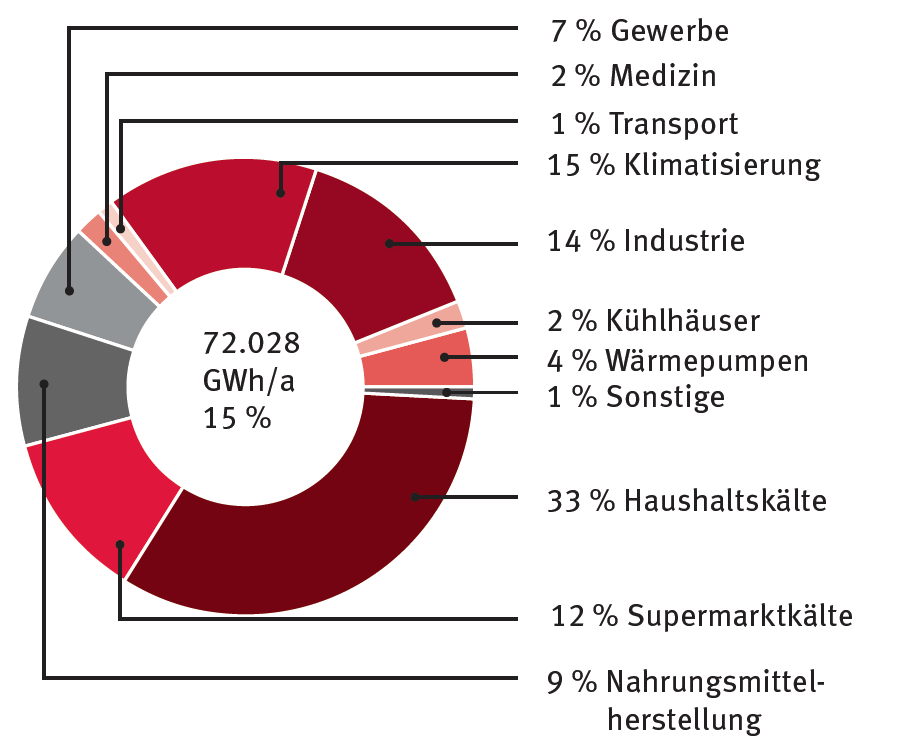
\includegraphics[width=0.570\textwidth]{Pictures/Energieverbrauch_Aufteilung_Karlsruhe.png}
	\caption{Aufteilung der sich in Deutschland in Betrieb befindenden Kältemaschinen je nach Einsatzgebiet und Energieverbrauch im Jahre 2009. \citep{M.Stoeckner2012} \citep{Preuss2011}}
	\label{fig:Aufteilung nach Einsatzgebiet}
\end{figure}

Der Kälteleistungsbedarf ist nach wie vor ansteigend, womit eine größere Klimabelastung einhergeht. Auf der einen Seite entsteht eine steigende CO$_{2}$-Belastung für die Bereitstellung der Antriebsenergie der Kältemaschinen. Auf der anderen Seite stellt die Belastung der Umwelt durch ungewollte direkte Kältemittelemissionen mit teils hohen CO$_2$-Äquivalenten eine Herausforderung dar.

Im Bezug auf Kältemaschinen werden in der Literatur eine Vielzahl an Möglichkeiten und Potentialabschätzungen zur Senkung des Energieverbrauches und der Umweltbelastung genannt. Von der Verwendung von natürlichem Kältemittel, Wärmerückgewinnung vom Verflüssiger sowie von Downsizing des Kompressors ist die Rede. Laut EnergieAgentur.NRW \citep{EnergieAgenturNRW2010} entfallen bei der elektrischen Leistungsaufnahme einer Kälteanlage im Kühlbetrieb durchschnittlich:

\begin{itemize}
	\item ca. 88 $\%$ auf den Kompressor,
	\item ca. 7 $\%$ auf den Verflüssiger,
	\item ca. 5 $\%$ auf den Verdampfer.
\end{itemize}

Die Energieverbrauch des Verflüssigers bzw. Verdampfers wird durch deren eingebauten Ventilator bestimmt. 
Folglich ist der Kompressor der größte Energieverbaucher in einer Kälteanlage. Um eine effiziente Kälteanlage zu betreiben, sollte die zu verrichtende Arbeit vom Kompressor so niedrig wie möglich gehalten werden.

Ziel dieser Arbeit ist der Aufbau, die Inbetriebnahme und erste Test für ein Messsystem, das sowohl Vereisungs- als auch Abtauversuche für verschiedene Luftkühler durchführen kann. Vereiste Luftkühler führen zu einem Leistungsabfall der Kälteleistung. \cite{Grote2014}Dadurch muss der Luftkühler zu bestimmten Zeiten abgetaut werden, um das Eis von dem Wärmeübertrager zu entfernen und die ursprüngliche Kälteleistung wieder zur Verfügung stellen zu können. 





\chapter{Motivation und Ziele}
\label{cha:Motivation_und_Ziele}

In diesem Kapitel wird die Motivation und die gesetzten Ziele der vorliegenden  Arbeit aufgezeigt.

Am \textit{Institute for Energy Efficient Buildings and Indoor Climate }(EBC) wird in Kooperation mit dem \textit{Lehrstuhl für Wärme- und Stoffübertragung }(WSA) verschiedene Abtaumethoden für vereiste Luftkühler erforscht. Der Auftraggeber und Kooperationspartner für die Forschungsarbeiten ist der \textit{Forschungsrat Kältetechnik e.V}. Die komplette Projektumgebung ist in der Abbildung \ref{fig:Projektumgebung} dargestellt

\begin{figure}[htb]
	\centering
		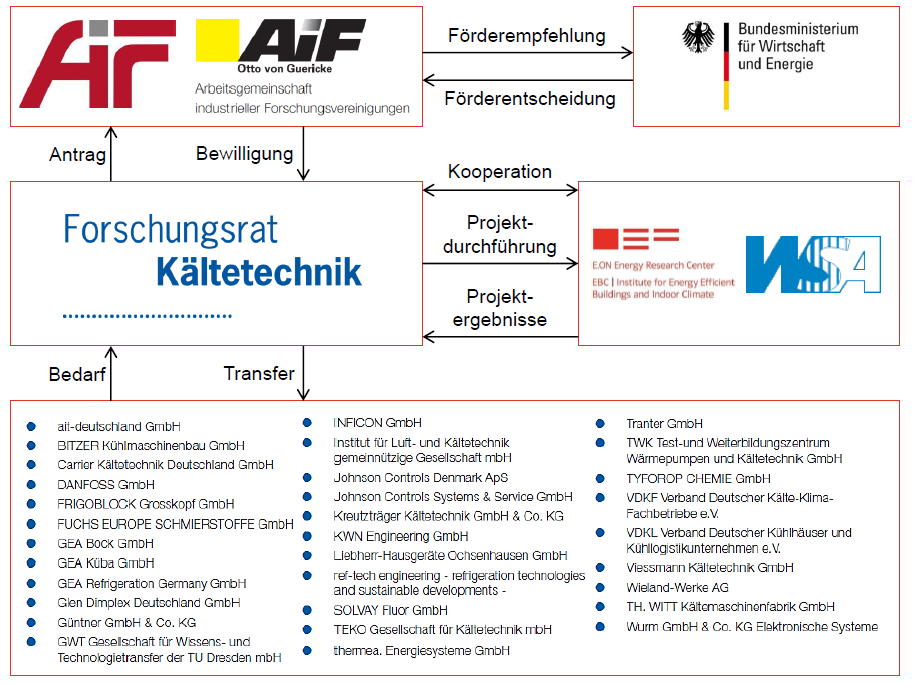
\includegraphics[width=0.80\textwidth]{Pictures/Projektumgebung.png}
	\caption{Projektumgebung für den EBC Abtauprüfstand \citep{Freitag2015}}
	\label{fig:Projektumgebung}
\end{figure}

Die Motivation zu diesem Forschungsprojekt rührt aus dem simplen Phänomen, dass bei der Unterschreitung des Taupunktes der zu kühlenden, vorbeiströmenden Luft zunächst eine Bereifung des Luftkühlers stattfindet. Die Bereifung führt bei einer Verdampfungstemperatur kleiner als 0 °C und somit Unterschreitung des Gefrierpunktes zu einer Vereisung. Die Bereifung führt durch Querschnittsverengungen im Wärmeübertrager des Luftkühlers zu einer erhöhten Strömungsgeschwindigkeit. Diese führt zunächst zu einem erhöhten Wärmeübergang und somit zu einer höhren übertragenden Leistung vom Luftkühler auf die Luft.\citep{Schydlo2010} 

Eine spätere Bereifung der Lamellen führt zu einem sinkenden Wärmeübergang zwischen der Lamelle und der Luft, da sich das gefrorene Eis aufgrund der geringen Wärmeleitfähigkeit wie ein Isolator verhält. Um den eintretenden Leistungsabfall zu kompensieren, wird die Regelung der Kälteanlage die Verdampfungstemperatur verringern. Eine geringere Verdampfungstemperatur bedeutet einen geringeren Betriebssaugdruck, den der Kompressor bereitstellen muss. Eine höhere Druckdifferenz führt zu einem erhöhten Stromverbrauch und gleichzeitig sinkt der Wirkungsgrad der gesamten Kälteanlage.
Aus dieser Kausalkette sollte eine Kälteanlage im Falle einer Vereisung abgetaut werden, um danach wieder seine Nennleistung zu Verfügung stellen zu können.

 \begin{figure}[htb]
	\centering
		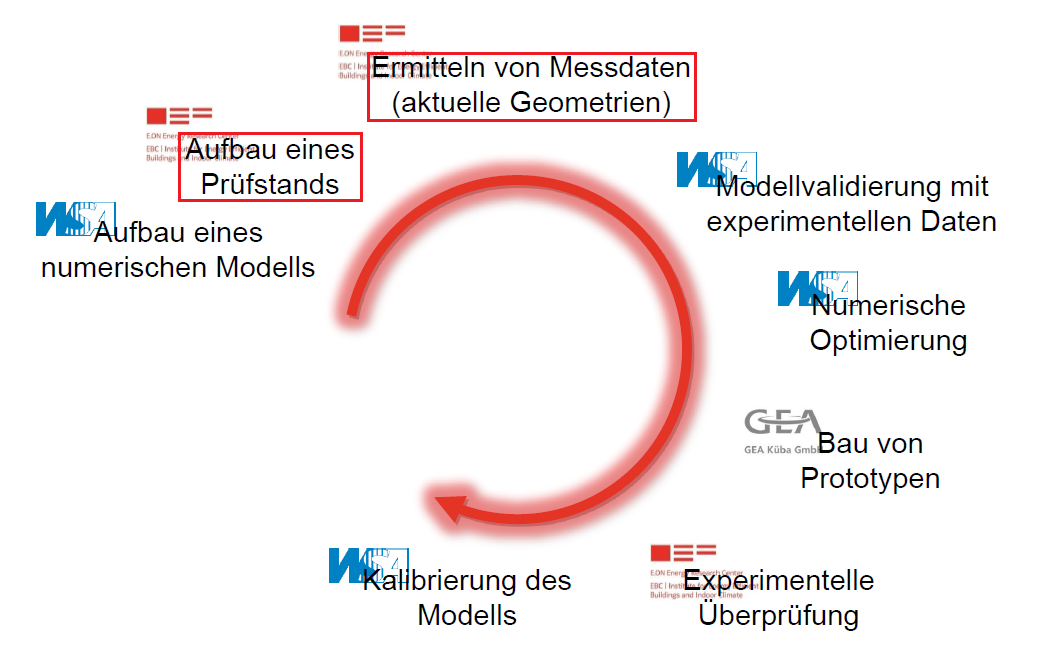
\includegraphics[width=0.80\textwidth]{Pictures/Projektablauf.png}
	\caption{Aufgabenpakete im Projektzyklus.\citep{Freitag2015} Rot umrahmte Arbeitspakte werden in dieser Masterarbeit behandelt und durchgeführt.}
	\label{fig:Aufgabenpakete}
\end{figure}

Die Ziele dieses Forschungsvorhabens sind sowohl experimentelle als auch numerische Erkenntnisgewinne im Hinblick auf Reifbildungsvorgänge als auch verschiedener Abtaumethoden bei Luftkühlern in einem Kältekreislauf. Diese Erkenntnisse sollen in eine spätere Datenbasis fließen, die zur energieeffizienten Auslegung von Luftkühlerkomponenten dienen wird.

Das WSA übernimmt hierbei die Entwicklung eines numerischen Simulationsmodelles. Das EBC ist verantwortlich für den Aufbau eines Abtauprüfstand zur Validierung der Simulationsergebnisse. Hierzu wurde bereits in einer vorhergegangenen Masterarbeit von \citeauthor{Helmlinger2015} eine Kälteanlage geplant und in Betrieb genommen. Der Luftkühler ist hierbei in einer Klimakammer platziert, in der unterschiedlichste Raumbedingungen eingestellt werden können. Die Luftkühler können getauscht werden, um verschiedene Wärmetauscher-Varianten testen zu können.

Diese Masterarbeit umfasst, wie in Abbildung \ref{fig:Aufgabenpakete} dargestellt, die Arbeitspakete 

\begin{itemize}
\item	Aufbau (bzw. Optimierung) eines Prüfstandes
\item	Ermitteln von Messdaten.
\end{itemize}

Das Arbeitspaket \textit{Aufbau (bzw. Optimierung) eines Prüfstandes} unterteilt sich in 

\begin{itemize}
\item Entwicklung und Bau eines Wägesystems zur Messung und Bestimmung des 2D-Schwerpunktes der Eismenge im Luftkühler
\item Entwicklung und Implemtierung einer Speicher-Programmierbaren-Steuerung
\end{itemize}





\chapter{Grundlagen}
\label{cha:Grundlagen}



In diesem Kapitel werden die  theoretischen Grundlagen für diese Arbeit erläutert. 
Zuerst wird in Abschnitt \ref{sec:Thermodynamik} die thermodynamischen Grundlagen vorgestellt, um dann in Abschnitt \ref{sec:Kaeltetechnik} näher auf die kältetechnischen Grundlagen einzugehen. 


\section{Kaltdampf-Kälteprozesses}
\label{sec:Thermodynamik}

\subsection*{Thermodynamik}
Ein Verdampfer hat die Aufgabe, einer Umgebung Wärme zu entziehen. Hierfür wird in einem Wärmeübertrager flüssiges Kältemittel verdampft. Das verdampfende Kältemittel kühlt zunächst den Wärmeübertrager, danach wird über die Wärmeübertrager-Lamellen der vorbei strömende Luft Wärme entzogen.
Der Kaltdampf-Kälteprozess ist ein linksläufiger \textit{Clausius-Rankine-Kreisprozess}. Die Zustandspunkte des verwendeten Kältemittels im log p,h Diagramm sind in Abbildung \ref{fig:Komponenten} dargestellt. 

\begin{figure}[htb]
\centering		
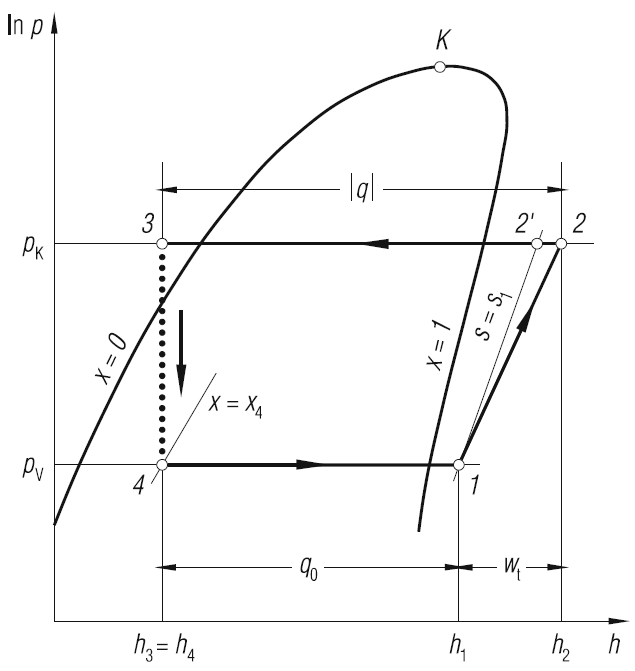
\includegraphics[width=0.6\textwidth]{Pictures/log_p_h_Beahr.png}
\caption{Kreisprozess im log p,h-Diagramm \citep{Baehr2013}}
\label{fig:Komponenten}
\end{figure}


Das halb-logarithmische Diagramm ist ein vielgebrauchtes und hilfreiches Mittel in der Kältetechnik. 
\footnote{Das Zustandsdiagramm wurde vom deutschen Ingenieur Richard Mollier (1863-1935) im Jahre 1924 erstmalig vorgestellt.} 
Der Druck ist logarithmisch auf der y-Achse und die spezifische Enthalpie $h$ auf der x-Achse eingetragen. Es gibt drei Gebiete im Diagramm: flüssiges Kältemittel, gasförmiges überhitztes Kältemittel und das Nassdampfgebiet. Im Nassdampfgebiet liegt ein Gemisch aus gasförmigen und flüssigem Kältemittel vor. Der Anteil des Gases im Nassdampfgebiet wird durch $x$ ausgedrückt; $1-x$ ist der Anteil der Flüssigkeit.


Im Diagramm \ref{fig:Komponenten} sind alle Zustandspunkte des Kältekreislaufes abgebildet. 
Innerhalb des Nassdampfgebietes führt Wärmezu- oder abfuhr  nicht zu einer Erhöhung der Temperatur, sondern zu einer Veränderung vom Gas- bzw. Flüssigkeitsanteil. Es wird von einer \textit{latenten}, also nicht fühlbaren,  Wärmeänderung gesprochen. 
%Um einen Tropfen flüssigen Wasser, dessen Zustand sich auf der Siedelinie befindet, in einen gasförmigen Zustand, sprich $x=1$ zu überführen, muss ihm die spezifische Verdampfungsenthalpie $\Delta h$ zugeführt werden. Verläuft die Zustandsänderung entgegengesetzt, kondensiert der Tropfen und gibt die Verdampfungsenthalpie $\Delta h$ an seine Umgebung ab. 
Außerhalb des Nassdampfgebietes führt eine Wärmezu- oder abfuhr zu einer Veränderung der Temperatur. Die Wärmeänderung ist \textit{sensibel}. 


Ein Kreisprozess kann in folgende vier Prozessschritte unterteilt werden:

\begin{tabular}{p{1.5cm}p{13cm}ll}
\hline
\textbf{1 $\longrightarrow$ 2} & Kompression des dampfförmigen Kältemittels durch mechanische Leistungszufuhr  \\ 
\hline
\textbf{2 $\longrightarrow$ 3} & Abkühlung, Kondensation und Unterkühlung des Kältemittels durch Abgabe vom Wärmestrom $\dot{Q}$ über den Verflüssiger an die Umgebung \\ 
\hline
\textbf{3 $\longrightarrow$ 4} & Entspannung des flüssigen Kältemittels durch das Drosselventil; teilweise setzt die Verdampfung des Fluids ein \\ 
\hline

\textbf{4 $\longrightarrow$ 1} & Verdampfung des noch flüssigen Kältemittels auf niedrigem Druckniveau unter der Aufnahme des Wärmestromes $\dot{Q_0}_0$ aus dem Kühlraum \\ 
\hline
&\\
\end{tabular}
\hspace{1cm}

Der Prozess findet auf zwei Druckniveaus statt: dem Verdampfungsdruck $p_V$ und dem Kondensationsdruck $p_K$. Die Verflüssigung des Kältemittels findet auf hohem Druckniveau und die Verdampfung auf niedrigem Druck statt. Die höchste Temperatur wird nach der Kompression am Zustandspunkt 2 erreicht; er befindet sich im überhitzten Gasgebiet. Die niedrigste Temperatur ist kurz nach dem Dosselventil und vor dem Verdampfer am Punkt 4. auf niedrigem Druckniveau. 

Nach dem Anwenden des 1. Hauptsatzes der Thermodynamik (\textit{Erhaltung der Energie in einem System}) auf den Kältekreislauf folgt die Gleichung :

 \begin{equation}
 	|\dot{Q}|  = \dot{Q_0} +  P_{KM}.
 	\label{eq:Energiebilanz}
 \end{equation}
 
Die elektrische Antriebsleistung der Kältemaschine ist die aufgenommene elektrische Leistung durch den Kompressor zwischen den Zustandspunkten 1  und 2, geteilt durch den mechanischen und elektrischen Wirkungsgrad des Elektromotors. Sie ergibt sich zu:

\begin{equation}
P_{KM} = \frac{\dot{m}~ w_t}{\eta_{el} \cdot \eta_{mech}}= \frac{\dot{m}}{{\eta_{el} \cdot \eta_{mech}}}~ (h_2 - h_1) = \frac{\dot{m} }{\eta_{sV}\eta_{el} \cdot \eta_{mech}} (h_{2'}- h_1).
\label{eq:Antriebsleistung}
\end{equation}

Hierbei ist $\eta_{sV}$ der isentrope Wirkungsgrad des Kompressors. Der isentrope Wirkungsgrad setzt den realen Kältekreislauf in ein Verhältnis zum idealen Kältekreislauf. Die Überhitzung des Gases am Austritt des Kompressors ist höher als die Überhitzung nach einer isentropen Verdichtung. Daraus folgt eine höhere Leistungsaufnahme durch den Kompressor und ein höherer Wärmestrom $\dot{Q}$, der über den Verflüssiger an die Umgebung abgegeben werden muss. Der isentrope Wirkungsgrad ist definiert über 

\begin{equation}
\eta_{sV}:= \frac{h_{2'}- h_{1}}{h_2 - h_1}.
\label{eq:Antriebsleistung}
\end{equation}


Der Wärmestrom $\dot{Q}$ wird über den Verflüssiger zwischen den Zuständen 2 und 3 abgeführt. Die Formel von  $\dot{Q}$ lautet: 

\begin{equation}
	\dot{Q} = \dot{m}~q_0 = \dot{m}~ (h_3 - h_2)< 0.
	\label{eq:Wärmestrom}
\end{equation}

Der Wärmestrom $\dot{Q}$ ist immer kleiner als Null; er wird dem Kreislauf folglich entzogen.  
 
Über ein Drosselorgan wird das Kältemittel vom hohen Druckniveau auf das niedrigere Druckniveau entspannt. Der Teilprozess findet zwischen den Zustandspunkten 3 und 4 statt und wird als \textit{isenthalp} angenommen.  
 
Die Kälteleistung $\dot{Q_0}$, der aus dem Kühlraum zu entnehmende Wärmestrom, ergibt sich aus dem Kältemittel-Massenstrom $\dot{m}$ und den spezifischen Enthalpien der Zustände 4 und 1 :

\begin{equation}
	\dot{Q_0} = \dot{m}~ q_0 = \dot{m}~ (h_1 - h_4).
	\label{eq:Kälteleistung}
\end{equation}




Die Bewertung einer Kälteanlage erfolgt durch die Leistungszahl $\epsilon_{KM}$: 

\begin{equation}
	\epsilon_{KM} := \frac{Kälteleistung}{Antriebsleistung} =\frac{\dot{Q_0}}{P_{KM}}.
	\label{eq:Leistungszahl}
\end{equation}


%
\subsection{Reif- und Eisbildung}
\label{subsec:Reifbildung}

Liegt die Oberflächentemperatur auf dem Wärmeübertrager des Verdampfers nicht nur unter dem Taupunktpunkt der feuchten Luft, sondern auch unter dem Gefrierpunkt, kann es zum Gefrieren der kondensierten Tropfen und/oder zur Desublimation von Wasserpartikeln auf der Oberfläche kommen. Dieser Abschnitt soll einen Überblick über diese zwei thermodynamischen Phänome geben. Da in dieser Arbeit nicht der Reifbildungsprozess im Hauptfokus steht, sondern  der technische Aspekt der Abtauung, wird der Eisbildungsprozess hier nur kurz erläutert.

In der Literatur gibt es zahlreiche Quellen, die sich mit der Reif- bzw. Eisbildung auseinander setzen. Die Quellen beschreiben den Kristallbildungsprozess sowohl aus der rein theoretischer Sicht als auch mittels simulationsrelevanten und technischen Überlegungen bzw. Untersuchungen. Der scheinbar triviale Prozess der Bildung eines Eiskristalles auf einer Oberfläche und sein weiteres Wachstumsverhalten ist sehr komplex und Gegenstand zahlreicher aktueller und schon abgeschlossener Forschungsprojekte.

Neben den theoretischen Grundlagen wird in der Arbeit von \textsc{\citeauthor{Schydlo2010}} ein Simulationsmodell für den Reifbildungs- und Abtauprozess auf einem Rohr entwickelt. Zudem sind bisherige Arbeiten zu der Thematik in \citep{Schydlo2010} aufgelistet und zusammengefasst. 
Praktische Untersuchungen sowie Versuchsaufbauten zum Thema der Vereisung von Luftkühlern werden in \textsc{\citeauthor{Sahinagic2004}} und \textsc{\citeauthor{Kosowski2009}} beschrieben. In den Arbeiten werden die Vereisungs- und innovative Abtauungsprozesse von einer CO$_2$-Wärmepumpe, die zur Heizung von Passivhäuser eingesetzt wird, untersucht.   



Es gibt zahlreiche Einflussgrößen, die auf den Prozess und die Form des Eiskristalls und späteren Reif einwirkten. 
  Die wichtigsten Einflussgrößen sind die Luftgeschwindigkeit, die Lufttemperatur, die Luftfeuchte, die Oberflächentemperatur und die Zeit. Um den Reif charakterisieren zu können, werden folgende Größen zur Hilfe genommen: die Reifdicke, die Reifdichte, die Porösität und die Wärmeleitfähigkeit. 

In der Arbeit von \textsc{\citeauthor{Hayashi1977}} aus dem Jahre 1977 wird der Eiskristallwachstum in drei Phasen unterteilt:

\begin{enumerate}
\item Eindimensionales Kristallwachstum
\item Reifschichtwachstumsphase 
\item Vergletscherung.
\end{enumerate}


\begin{figure}[htb]
\centering		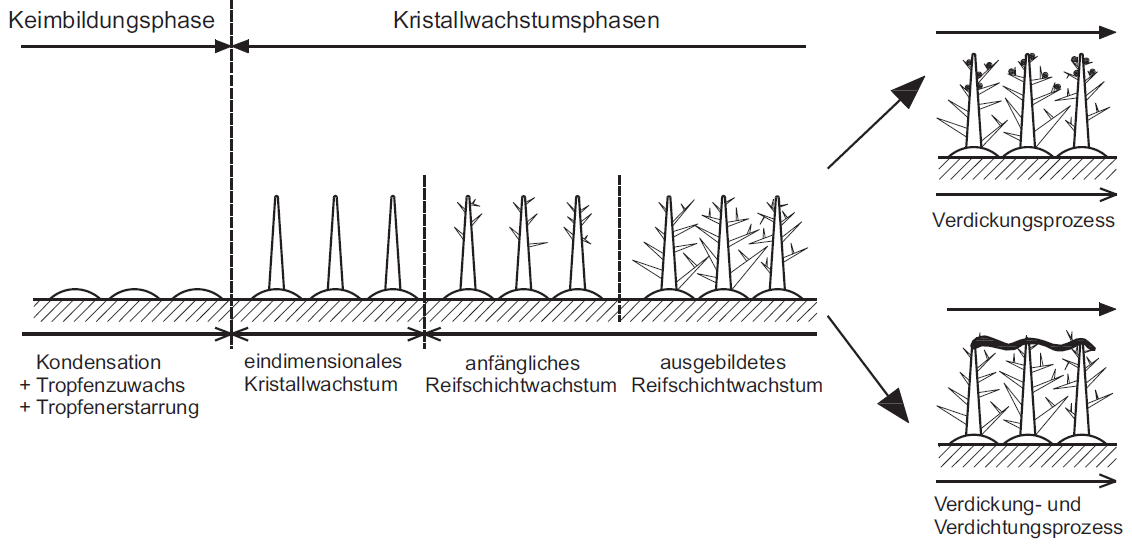
\includegraphics[width=0.85\textwidth]{Pictures/Reifbildungsphasen_Schydlo.png}
\caption{Kristallwachstum auf einer ebenen Oberfläche \citep{Schydlo2010}}
\label{fig:Kristallwachstum}
\end{figure}


In Abbildung \ref{fig:Kristallwachstum} sind die drei Kristallwachstums-Phasen nach \textsc{\citeauthor{Hayashi1977}} sowie die vorhergehende Keimbildungsphase, eingeführt in \citep{Sahinagic2004}, dargestellt. 

\subsubsection*{Keimbildungsphase}

In der Keimbildungsphase bilden sich zunächst Wassertropfen auf der Lamellenoberfläche, die trotz Temperaturen kleiner als der Gefrierpunkt nicht erstarren, sondern zu größeren Tropfen anwachsen. Je kleiner die Unterkühlung, desto größer werden die Tropfen, bevor sie erstarren und in die erste Kristallwachstumsphase übergehen. 

\subsubsection*{Eindimensionales Kristallwachstum}
Die erste Phase ist gekennzeichnet durch Kristallwachstum senkrecht zur Oberfläche und mit einheitlicher Wachstumsgeschwindigkeit. Dies führt aufgrund der sich stetig vermehrenden Kristalle zu einer erhöhten Rauigkeit.  

\subsubsection*{Reifschichtwachstumsphase}
In der zweiten Phase beginnt das dreidimensionale Wachstum. Die Kristalle fangen an sich miteinander zu verästeln. Ein poröses Kristallgitter entsteht. Aufgrund des  Wärmeleitwiderstandes, der mit der Reifdicke steigt, erhöht sich die Oberflächentemperatur der Reifschicht. Des weiteren kommt es zu einem Massenstrom innerhalb der Reifschicht, ausgelöst durch Diffusion. Die Diffusion rührt aus  dem  Konzentrationsunterschieden zwischen der Lamelle und der Reifoberfläche. Der Wassermassenstrom läuft in das poröse Kristallgitter und gefriert dort in Nähe der Lamelle. Die Dichte der Reifschicht steigt und mit ihr der Wärmewiderstand. Dies führt zu einer Erhöhung der Oberflächentemperatur der Reifschicht und schließlich zur Überschreitung des Gefrierpunktes von Eis. Die Spitzen des Kristalle schmelzen und es bildet sich Kondensat. Die dritte Wachstumsphase beginnt. 

\subsubsection*{Vergletscherung}

Das flüssige Wasser läuft aufgrund der Kapillarwirkung der Kristalle in die Zwischenräume des Kristallgitters und gefriert dort wieder. Die Kristallgitter werden dichter und kompakter. Dies führt zur Steigerung der Wärmeleitfähigkeit der Reifschicht. Es wird von einer Vergletscherung gesprochen. Die Oberflächentemperatur der Reifschicht sinkt erneut und fällt erneut unter den Gefrierpunkt. Nun kann die feuchte Luft erneut an der Oberfläche des Reifs desublimieren. Der Prozess wiederholt sich solange, bis das Eis so kompakt ist, dass kein weiteres Kondensat mehr in die Reifschicht eindringen kann. 

\subsection*{Physikalische Eigenschaften von Eiskristallen}

 Im vorangegangenen Abschnitt \ref{subsec:Reifbildung} wurden die einzelnen Bildungsphasen von Eiskristallen beschrieben. In diesem Abschnitt wird auf die Eigenschaften von Eiskristallen eingegangen und dargestellt wie sie sich während eines Vereisungsvorganges eines Luftkühlers verändern. 
 
Gefriert ein Tropfen Wasser und wird zum Eiskristall, so verändern sich die physikalischen Eigenschaften des Tropfens. In der Arbeit von \textsc{\citeauthor{Schydlo2010}} verdeutlichen zunächst zwei Diagramme, abgebildet in \ref{fig:Zeitverlaufe von Reifdichte und -dicke}, wie sich die Reifdicke und die Reifdichte während eines Vereisungsvorgang verändern. 

\begin{figure}
\centering
    \subfigure[Reifdichte]
    {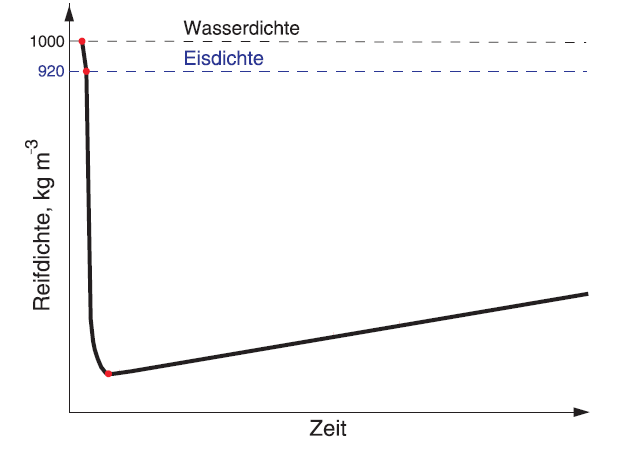
\includegraphics[width=0.50\textwidth]{Pictures/Reifdichte_Schydlo.png}}
    \subfigure[Reifdicke]{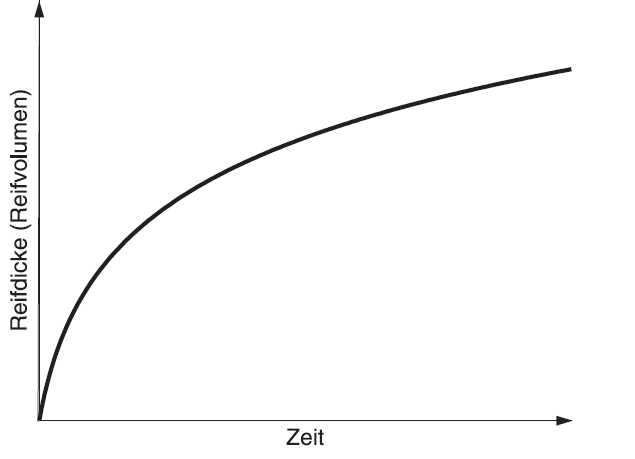
\includegraphics[width=0.48\textwidth]{Pictures/Reifdicke_Schydlo.png}}
\caption{Schematischer Reifdichte- und Reifdickeverläufe beim Vereisungsvorgang eines Tropfen Wassers \cite{Schydlo2010}}
\label{fig:Zeitverlaufe von Reifdichte und -dicke}
\end{figure}

Da Diagramm \ref{fig:Zeitverlaufe von Reifdichte und -dicke}(a) zeigt den Dichteverlauf, aufgetragen über die Vereisungszeit. Die Dichte eines Tropfens fällt beim Gefrieren von 1000 kg/m$^3$ auf 920 kg/m$^3$ sinkt. Danach tritt das in Abschnitt \ref{subsec:Reifbildung} beschriebene eindimensionale Wachstum ein, sodass die Reifdichte bis auf ein Minimum fällt. Danach tritt die dreidimensionale Wachstumsphase und dann die Vergletscherungsphase ein. Die Dichte  steigt jetzt langsam, aber kontinuierlich wieder an.

\begin{figure}[htb]
\centering	
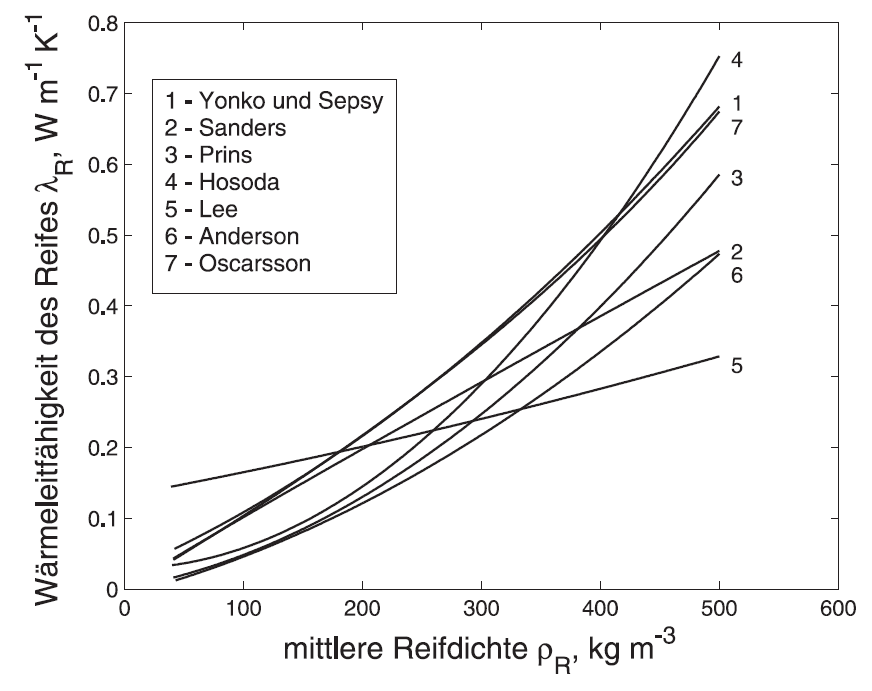
\includegraphics[width=0.55\textwidth]{Pictures/Waermeleitfaehigkeit_Schydlo.png}
\caption{Wärmeleitfähigkeit des Reifs aufgetragen über die mittlere Reifdichte \citep{Schydlo2010}}
\label{fig:Waermeleitfaehigkeit}
\end{figure}

Im \ref{fig:Zeitverlaufe von Reifdichte und -dicke}(b) ist der Reifdickenverlauf aufgetragen. Aus diesem lässt sich entnehmen, dass kurz nach Beginn die zeitliche Änderung der Reifdicke maximal ist. Das heißt, dass der Massenstrom an Kondensat, das sich an der Lamelle absondert und dann gefriert, am Anfang am größten ist und findet während des eindimensionalen Wachstums auf statt. Beim dreidimensionalen Wachstum und späteren Vergletscherung flacht die Kurve ab und strebt gegen einen Sättigungswert. 


 
Mit der Reifdicke verändert sich wiederum die Wärmeleitfähigkeit des Reifes, abgebildet in \ref{fig:Waermeleitfaehigkeit}. In dem Diagramm sind mehrere Berechnungsmodelle aufgetragen, die die Wärmeleitfähigkeit als Funktion der mittleren Reifdichte abbilden. Alle Modelle sagen einen Anstieg von $\lambda$ mit steigender Reifdichte voraus. Dies hängt mit der Verdichtung des Eises während der Vergletscherungsphase zusammen. Die führt dazu, dass Reif mit einer geringen Dichte gleichzeitig als sehr guter Isolator fungiert. \citep{Baehr2013}  \citep{Kosowski2009}





\section{Kältetechnik}
\label{sec:Kaeltetechnik}

Die Kältetechnik wird in verschiedensten Einsatzgebieten eingesetzt, um Kälte zu erzeugen bzw. einem definierten Raum Energie in Form von Wärme zu entziehen. 

Das Konservieren von Lebensmittel ist  der ursprüngliche Hauptzwecke der Kältetechnik und ist auch heute noch aktuell. Bereits 3000 Jahre v. Chr. nutzten die Ägypter und Mesopotamier Natureis, um ihre Nahrungsmittel länger haltbar zu machen.\citep{Danfoss2006}

Im Jahre 1834 meldete der US-Amerikaner Jacob Perkins sein Patent zum Thema Kältetechnik in England an. Das Patent beschreibt eine Kaltdampfmaschine in einem geschlossenen Kreislauf mit dem feuergefährlichen Äthyläther als Kältemittel.\citep{Siemens2007}

Carl von Linde baute nach konstruktiven Verbesserungen der Kaltdampfmaschine und Verwendung von Ammoniak als Kältemittel im Jahre 1876 die erste praxistaugliche Kälteanlage. Die ersten Anlagen wurden durch die Maschinenfabrik Augsburg-Nürnberg gebaut und an Brauereien sowie später auch an die Schifffahrt vertrieben.

Mit steigender Bedeutung von Elektrizität als Energieträger nach dem 1.Weltkrieg nahm auch die Entwicklung und der Bedarf an Kälteanlagen zu. Im Jahre 1920 startet die Firma \textit{General Electric} mit der Serienherstellung von Haushaltkühlschränken mit Hermetik-Verdichtern.

Das vielseitige Gebiet der Kältetechnik umfasst alle Technologien, die zur Bereitstellung von Kälteenergie dienen. Sie unterscheiden sich in der benötigten zuzuführenden Energien, Einsatzbereich und eingesetzten Kältemitteln.  Zu den wichtigsten und heute meist verwendeten Technologien gehören folgende Technologien

\begin{itemize}

\item Kompressions-Kälteprozess: \textit{Prozess wird angetrieben durch Zufuhr mechanischer Energie}
\item Sorptions-Kälteprozess: \textit{Prozess wird angetrieben durch Zufuhr von Wärmeenergie}
\item Linde-Verfahren.

\end{itemize}

Weitere nicht so weitverbreitete Technologien der Kältetechnik, jedoch technisch interessante Verfahren  sind zB. das  \textit{Wirbelrohr},  \textit{Magnetische Kühlung} oder das Kühlen mittels einem Peltier-Element. Diese Verfahren werden meist nur unter hohem Energieverbrauch in Sonderfällen angewandt. \citep{Grote2014}

Da sich diese Masterarbeit mit dem Aufbau eines Prüfstandes zur Untersuchung von Abtaumethoden einer Kompressionskälteanlage beschäftigt, wird in den folgenden Kapitel ausschließlich auf diese Technologie eingegangen. Für weitere Informationen bezüglich der anderen Technologien sei an dieser Stelle auf die Literatur \citep{Baehr2013}, \citep{Grote2014} und \citep{Grote2014} verwiesen.



\subsection{Komponenten eines Kaltdampfprozesses}
\label{subsec:Komponenten eines Kaltdampfprozesses}

Die Komponenten für einen einfachen Kaltdampfprozess  besteht aus vier Komponenten:

\begin{itemize}
\item der Kompressor
\item der Verflüssiger 
\item das Drosselvenil Expansionsventil
\item der Verdampfer. 
\end{itemize}

In Abbildung \ref{fig:einfacher Kältekreislauf} sind die vier Komponenten mit ihren Zustandspunkten dargestellt.

\begin{figure}[htb]
\centering		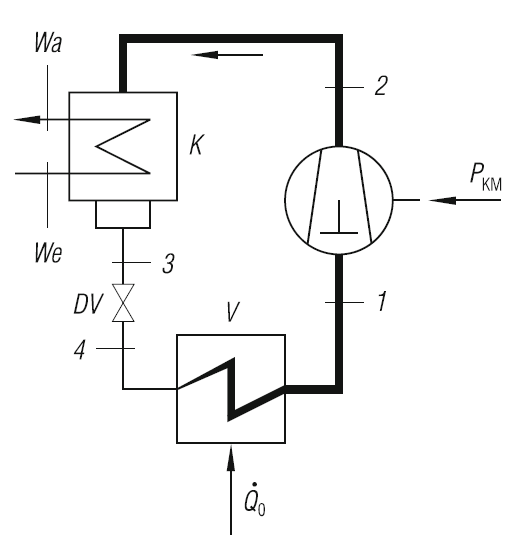
\includegraphics[width=0.50\textwidth]{Pictures/Kaltekreislauf_beahr.png}
\caption{Einfacher Kältekreislauf \citep{Baehr2013}}
\label{fig:einfacher Kältekreislauf}
\end{figure}

\subsubsection*{Der Kompressor}
Der Kompressor bildet das Herzstück der Kälteanlage. Er verdichtet das gasförmige Kältemittel von niedrigem Druck auf ein höheres Druckniveau. Um diese Arbeit zu verrichten, wird der Verdichter mit elektrischer Energie versorgt. Der Kompressor gibt es in verschiedenen Bauvarianten. Die zwei wichtigsten Bauvarianten sind der \textit{Hubkolbenverdichter} und der \textit{Rotationskolbenverdichter}. Die Baugruppen der Verdichter werden in offene, halbhermetische und vollhermetische Verdichter unterschieden. Schrauben-,Scroll- sowie Turboverdichter sind Bauarten der \textit{Rotationskolbenverdichter}. 



Ein wichtiges Kriterium bei Verdichtern ist das Druckverhältnis von Ansaugdruck, vor der Kompression, und dem Ausgangsdruck. Das Druckverhältnis $\pi$ ist definiert als:



\begin{equation}
\pi := \frac{p_{aus}}{p_{ein}}.
\label{Druckverhältnis}
\end{equation}

\subsubsection*{Der Verflüssiger}

Dem Kältemittel wird im Verflüssiger auf einem hohen Druckniveau Wärme entzogen. Der Verflüssiger kühlt das überhitzte, gasförmige Kältemittel ab. Beim Austritt aus dem Verflüssiger ist das Kältemittel meist vollständig kondensiert. 
Um einen Wärmeentzug zu bewerkstelligen gibt es drei Bautypen:

\begin{itemize}
\item Wassergekühlte Verflüssiger
\item Luftgekühlte Verflüssiger
\item Verdunstungsverflüsssiger
\end{itemize}

Wassergekühlte Verflüssiger können, aufgrund der besseren Wäärmeübertragung verglichen zu Luft, sehr kompakt gebaut werden. Eine typische Bauform ist das \textit{Bündelrohrverflüssiger}.
In der Praxis werden am häufigsten luftgekühlte Verflüssiger eingesetzt. Um die gleiche Kühlleistung wie ein wassergekühlter Verflüssiger zu erreichen, werden Lamellen und Ventilatoren eingesetzt. Die Lamellen vergrößern die Fläche für die Wärmeübertragung mit der Luft. Ventilatoren ermöglichen durch einen höheren Luftdurchsatz und der daraus resultierendem höhere Wärmeübertragung eine größere Kühlleistung und eine kompaktere Bauform der Wärmeübertragers. Diese Variante hat den Vorteil, dass die einen wartungsfreien Betrieb  sowie eine einfache Reinigung ermöglicht.


\subsubsection*{Das Expansionsventil}

Das Expansionsventil versorgt den Verdampfer mit dem nötigen Kältemittel-Massenstrom. Die Zuführung des Kältemittels erfolgt über eine Druckdifferenz. Durch eine lokale Verengung des Strömungquerschnitts, verringet sich der Druck des durchfließenden Kältemittels. Das Kältemittel vergrößert sein Volumen und es kommt zur Expansion. Die Druckreduzierung erfolgt ohne zusätzliche Arbeit. Im idealen Fall wird bei diesem Prozess auch keine Wärme abgefuhrt; der Prozess ist \textit{isenthalb}. 
Das Expansionsventil trennt zusammen mit dem Kompressor die zwei Druckseiten des Kältekreislaufes. Es gibt Expansionsventile sowohl als regelbare und nicht regelbare Ausführungen. Bei kleineren Anlagen erfolgt die Expansion ungeregelt zum Beispiel durch Kapillarrohre. Geregelte Expansionsventile werden in mittleren und großen Kälteanlagen eingesetzt. Die Regelung erfolgt durch die Querschnittsänderung und dem damit einhergehendem Druckabfall.  

\subsubsection*{Der Verdampfer}

In dem Verdampfer wird das Kältemittel eingespritzt. Das Kältemittel verdampft und entzieht seiner Umgebung dabei Wärme. Aufgrund der vielfältigen Anforderungen an Verdampfer, gibt es eine Vielzahl an Bauarten für Verdampfer. Mögliche Bauarten sind 

\begin{itemize}
\item Glattrohrverdampfer
\item Beripptes Verdampferregister
\item Rippenrohrverdampfer
\end{itemize}

Um eine möglichst große Kälteleistung zu ermöglichen, werden wie beim Verflüssiger auch, Ventilatoren eingesetzt. Die Ventilatoren erzwingen einen Luftstrom durch den Verdampfer und erhöhen damit die Wärmeübertragung zwischen der Luft und den Verdampferrohren. 

%\newpage
\subsection{Abtaumethoden}
\label{subsec: Abtaumethoden}

Um einen vereisten Luftkühler abzutauen, gibt es mehrere Methoden. Die Methoden unterscheiden sich in der Installation, Schnelligkeit, Effizienz und Effektivität. Je nach Einsatzbereich und Anlage wird entschieden welche Abtaumethode installiert und eingesetzt wird. Mehrkosten für die Installation sowie weitere Betriebskosten sind bei der Entscheidung stets ein nicht zu vernachlässigender Punkt.
Die in der Praxis am weit verbreitesten Methoden sind  die \textit{Heißgas-Abtauung}, \textit{Prozessumkehrung}, \textit{elektrische Abtauung} und \textit{Umluft-Abtauung}.

Die Tabelle \ref{tab:Vor- und Nachteile} gibt einen Überblick über die Vor- und Nachteile der jeweiligen Abtaumethode. 

\subsubsection*{Heißgas-Abtauung}

Die Heißgasabtaung wird durchgeführt indem das Heißgas aus dem Kompressor anstatt in den Verflüssiger direkt in den vereisten Verdampfer leitet. Für diese Methode wird eine Bypass-Leitung von dem Austritt vom Verdichter bis zum Eingang des Expansionsventil gelegt. Mittels zwei Drei-Wegeventilen kann diese Leitung geöffnet bzw. geschlossen werden. In der Abtauphase ist der Verflüssiger vom Kreislauf ausgeschlossen, damit kein flüssiges Kältemittel in den Verdampfer fließt. \citep{Baehr2013}
Der Prozess läuft in 3 Schritten ab:

\begin{itemize}
\item[1$\longrightarrow$ 2] Kältemittel-Verdichtung durch den Kompressor unter Aufnahme elektrischer Energie

\item[2 $\longrightarrow$ 3] Isenthalpe Entspannung durch das Expansionsventil

\item[3 $\longrightarrow$ 1] Wärmeabgabe an Rohre, Lamellen und das Eis. 
\end{itemize}


In Abbildung \ref{fig:Heissgas-Abtauung} ist der rechtsläufige Kreisprozess in einem ln p, h- Diagramm für das Kältemittel R290 abgebildet. 


\begin{figure}[htb]
\centering
\subfigure[Fließbild. Links: Kühlbetrieb, Rechts: Abtaubetrieb]
{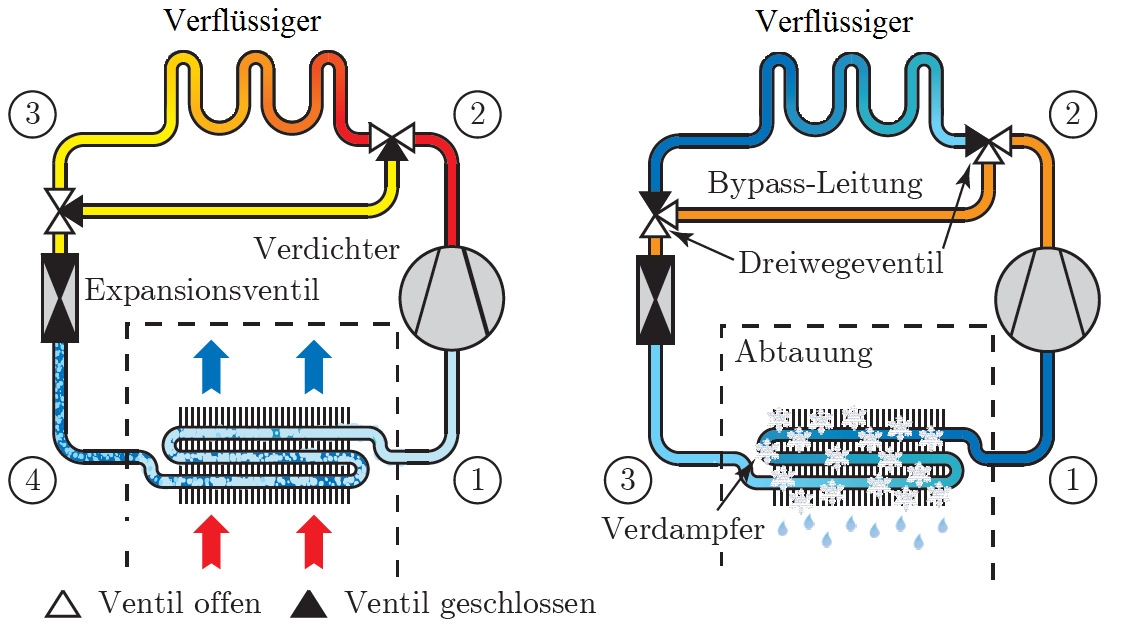
\includegraphics[width=0.640\textwidth]{Pictures/HeissgasKosowski.png}}
\subfigure[Zustandspunkte im ln p,h Diagramm]{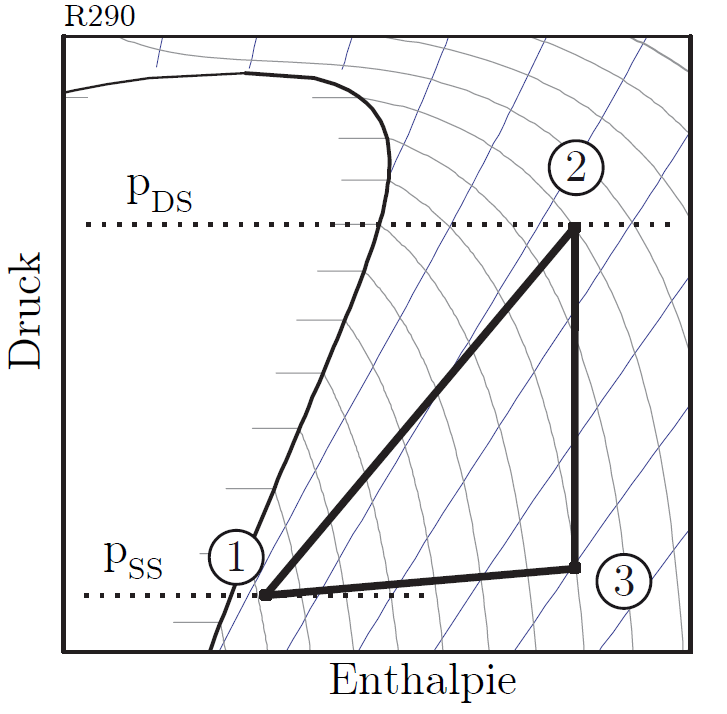
\includegraphics[width=0.35\textwidth]{Pictures/HeissgasEnthalpieDiagrammKosowski.png}}
\caption{Heißgas-Abtauung \citep{Kosowski2009}}
\label{fig:Heissgas-Abtauung}
\end{figure}



\subsubsection*{Prozessumkehrung}

Bei der Abtauung durch Prozessumkehrung wird die Funktion der Wärmeübertrager vertauscht. Während des Abtauprozesses fungiert der Verdampfer als Verflüssiger und der Verflüssiger hat die Aufgabe des Verdampfers inne. Die Prozessumkehrung wird in der Regel durch ein Vierwegeventil gewährleistet. Das Vierwegeventil wird bei der Abtauung geschaltet und leitet das Kältemittel nach dem Kompressor erst in den vereisten Verdampfer. Das überhitzte Kältemittel durchströmt den Verdampfer auf hohem Druckniveau und gibt Wärme an die Rohre und Lamellen des Luftkühlers sowie an das Eis ab.

Die Versuchsalage, die in dieser Arbeit optimiert worden ist, ist mit dieser Technologie ausgestattet. Der Umkehrprozess wird näher im Kapitel \ref{cha: Versuchsaufbau} erläutert. 


\begin{figure}[htb]
\centering		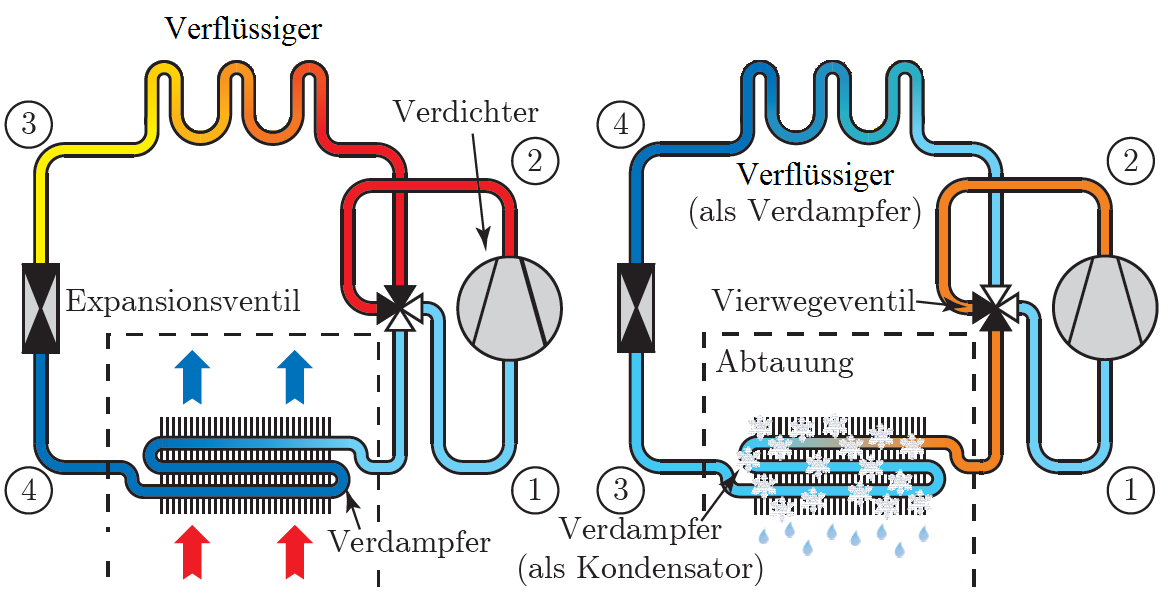
\includegraphics[width=0.7\textwidth]{Pictures/Prozessumkehrung_Kosowski.png}
\caption{Links: Kühlbetrieb. Rechts:Heißgas-Abtauung \citep{Kosowski2009}}
\label{fig:Prozessumkehrung}
\end{figure}

\subsubsection*{Elektrische Abtauung}

Eine weitere Möglichkeit der Abtauung ist die elektrische Abtauung. Bei dieser Methode sind Widerstandsheizungselemente in den Wärmeübertrager des Verdampfers installiert. Die Widerstandsheizung wandelt elektrische Energie in thermische Energie um, und überträgt diese weiter an den Wärmeübertrager und das Eis. 

Das Prinzip der Widerstandsheizung beruht auf einen niedrig ohmigen Widerstand, der von Strom durchflossen wird und sich dabei erhitzt. Die Widerstandsheizung, auch Heizpatronen genannt, können in Reihe oder auch parallel geschaltet werden. Bei der Erhitzung  Die abfallende elektrische Spannung über einen Heizswiderstand errechnet sich nach dem Ohmischen-Gesetz zu :

\begin{equation}
U = R I
\label{eq: Ohmisches Gesetz}
\end{equation}

Hierbei ist $R$ der spezifsche Widerstand des eingesetzen Material, meistens Metalle,  und $I$ die angelegte Stromstärke. Ein Heizwiderstand hat einen Wirkungsgrad von 100 $\%$ und wandelt somit die komplette elektrische Leistung in thermische um:

\begin{equation}
\dot{Q}_{th}= P_{el }= U I = \frac{U^2}{R} =  R I^2 
\label{eq:Leistung Heizwiderstand}
\end{equation}

Die thermische Leistung ist folglich proportional zu der angelegten Spannung $U$. Die Widerstände sind über die Spannung $U$ regelbar. Der Wärmeübergang von den Heizpatronen auf den Wärmeübertrager ist entscheidend für ein effizientes Abtausystem. Je formschlüssiger die Heizpatronen in den Verdampfer installiert sind, desto besser der Wärmeübergang und effizienter die Abtauuung.  
Die Versuchsanlage dieser Arbeit ist auch mit dieser Abtautechnologie ausgestattet. 

\subsubsection*{Umluft-Abtauung}

Die Umluft-Abtauung ist eine weitere in der Praxis häufig verwendete Abtaumethode. Hierbei wird der Verdampfer durch die vorbeiströmende Umluft abgetaut. Um dies zu ermöglichen muss zum einen der Ventilator in der Abtauphase laufen und zum anderen die Umgebungstemperatur größer als 0 $°$C sein. Ein Vorteil dieses Verfahrens ist, dass die Wärmeübertragung luftseitig geschieht und dadurch die zuzuführende Wärme nicht zusätzlich das Material des Verdampfers erhitzen muss. 

Diese Abtaumethode wird in der Arbeit nicht näher untersucht. Deswegen wird an dieser Stelle auf die  Literaturquellen \citep{Breidenbach2014} und \citep{Ehrbar2002} verwiesen. 

%\subsubsection{Gegenüberstellung der Abtaumethoden}
%\label{subsubsec:Gegenüberstellung }



%\begin{landscape}

\begin{table}%[htb]
\centering
\caption{Vor- und Nachteile der verschiedenen Abtaumethoden   	\citep{Breidenbach2014}, \citep{Refrigeration2000}, \citep{Yin2012}, \citep{Huang20091697}
} \vspace{6pt}

\label{fig:PCM_Slurry1}
%\begin{tabular}{p{3.9cm}p{8cm}p{8cm}lll} 
\begin{tabular}{p{3.8cm}p{5.6cm}p{5.6cm}lll}
\hline
\textbf{Abtaumethode} &\textbf{Vorteile} & \textbf{Nachteile}\\
\hline
\hline

\textbf{Heißgas-Abtauung} 
&
$\bullet$ Guter Wärmeübergang zwischen Heißgas,Rohre und Eis
\newline								  			
$\bullet$ Unkomplizierte Wartung
\newline			  
$\bullet$ Kurze Abtaudauer		
\newline			
$\bullet$ Schnelles Wiederanfahren möglich	

&$\bullet$ Höherer Planungs- und Installationsaufwand  
\newline
$\bullet$ Zusätzliche Kühlung des Kompressors in Abtauphase ist erforderlich 
\newline 
$\bullet$ Höhere Druckverluste durch zusätzliche Komponenten 
\newline
$\bullet$ kritische Kältemittel-Menge bestimmt durch Abtauleistung \\  
   
\hline
\textbf{Prozessumkehrung}
&$\bullet$ Guter Wärmeübergang zwischen Heißgas,Rohre und Eis  													
\newline								
$\bullet$ Unkomplizierte Wartung
\newline	
$\bullet$ Kurze Abtaudauer		
\newline			 
$\bullet$ geeignet für Verbund-Systeme		
&$\bullet$ Abtropfwanne ist nicht beheizt   
\newline
$\bullet$ Höherer Planungs- und Installationsaufwand
\newline
$\bullet$ Nicht nachrüstbar
\newline
$\bullet$ Höhere Druckverluste durch zusätzliche Komponenten								
\newline
$\bullet$ Kritische Kältemittel-Menge bestimmt durch Abtauleistung\\


\hline
\textbf{Elektrische Abtauung }
&$\bullet$ Einfache Komponenten und Installation 
\newline 
$\bullet$ \textit{Stand-Alone}-System ist nachrüstbar		
\newline
$\bullet$ Hohe Regelgenauigkeit	
\newline
$\bullet$ Abtropfwanne ist beheizbar 					
&
$\bullet$ Schlechter Wärmeübergang 
\newline					
$\bullet$ Verursacht Kältemittelbewegung in den Sammler
\newline 
$\bullet$ Brandgefahr im Falle von Kabelbruch  
\newline
$\bullet$ Zeitliche Verzögerung beim Abtauprozess 
\newline
$\bullet$ Hohe thermische Belastung der Komponenten    
\\

 
\hline
\textbf{Umluft-Abtauung }
&
$\bullet$	Keine zusätzlichen Komponenten nötig			 
\newline
$\bullet$	Günstig										
\newline
$\bullet$	Keine zusätzlicher Wärmeeintrag ins System	  
\newline
$\bullet$	Keine Abtauung der Abtauwanne möglich	
&
$\bullet$ Bei überdimensionierten Kompressoren sehr hohe Abtaudauer möglich
\newline
$\bullet$ Funktioniert nur mit Umgebungstemperaturen über $ 2\,^{\circ}\mathrm{C} $
\\
\hline

\end{tabular}
\label{tab:Vor- und Nachteile}
\end{table}
%\end{landscape}


\newpage
\section{Federn}
\label{sec:Federn}

Der Einsatzbereich von Federn ist genau so vielfältig wie die verschiedenen Bautypen, Größen und Werkstoffen. Je nach Funktion können Feder können zug-,druck-, torsion- oder biegebeansprucht werden. 
Die Hauptfunktionen umfassen die Gewährleistung des Kraftflusses und der Kraftverteilung, Speicherung von Energie, Ausdehnungsausgleich, Dampfungssysteme oder Schwingungssysteme. 
Federn werden charakterisiert durch ihre Feder-Kraft-Kennlinie bzw. Moment-Verdrehwinkel-Kennlinie. 

In dieser Arbeit wurde eine rechteckige Blattfeder dimensioniert, gefertigt und als Teil eines Wägesystems kalibriert, siehe Abschnitt \ref{sec:Waegesystem}. Deshalb werden in diesem Abschnitt nur auf biegebeanspruchte, rechteckige Blattfedern näher eingegangen. 

\begin{figure}[htb]
\centering
\subfigure[Rechteckblattfeder (Ansicht und Draufsicht)]
{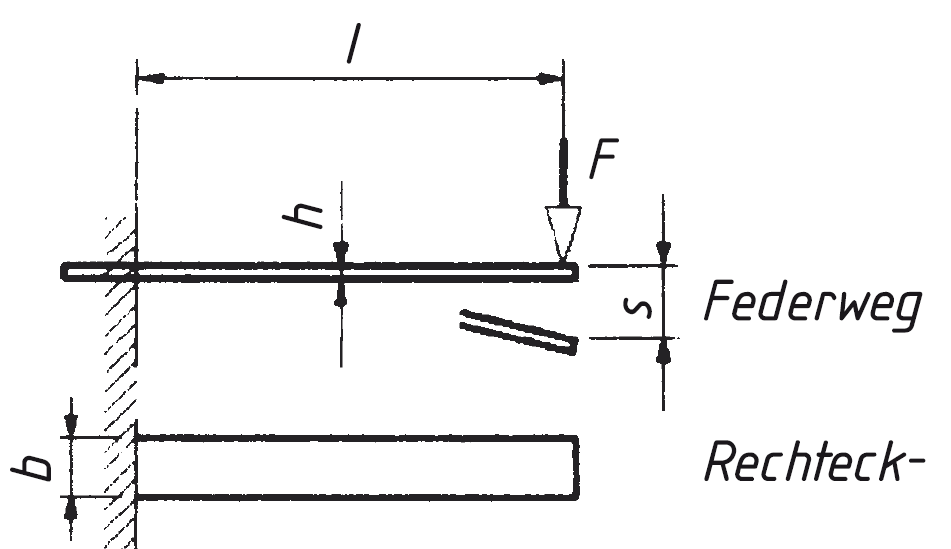
\includegraphics[width=0.4\textwidth]
{Pictures/Federprinzip.png}}
\subfigure[Kraft-Weg-Kennlinien]{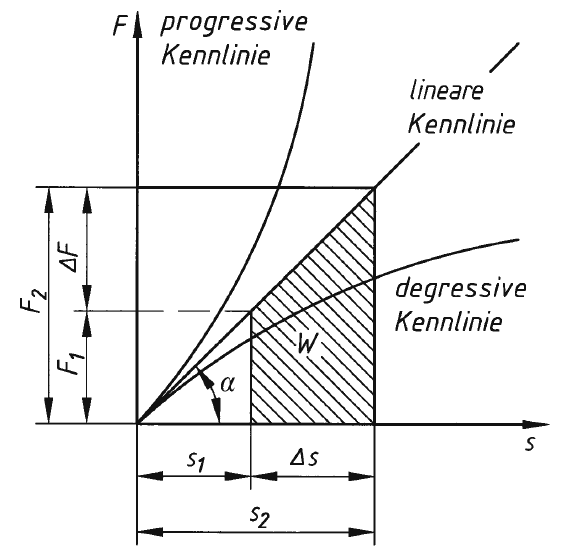
\includegraphics[width=0.4\textwidth]
{Pictures/Kraft-Weg-Kennlinie.png}}
\caption{Blattfeder und Feder-Kennlinien \citep{Wittel2011}}
\label{fig:Federdiagramm}
\end{figure}

Die Abbildung \ref{fig:Federdiagramm}(a) zeigt das Prinzip einer einsetig eingespannten, rechteckigen Blattfeder und \ref{fig:Federdiagramm}(b) drei unterschiedliche Kraft-Weg-Kennlinien. $l$ ist die Länge von der Einspannung bis zum Angriffspunkt der Kraft $F$. $h$ ist die Höhe und $b$ die Breite der Feder. Der Federweg $s$ resultiert aus der Verformung der Feder durch die Belastung mit der der Kraft $F$.

Eine rechteckige Blattfeder verhält sich bei Zunahme der belastenden Kraft $F$ , wie die $lineare~Kennlinie$ im Diagramm aufzeigt. Die Kraft $F$ und der Federweg $s$ sind zu einander proportional. Eine Verdoppelung der Kraft zieht gleichzeitig eine Verdoppelung des Federweges nach sich. Die meisten eingebauten Federn verfügen über eine solche lineare Kennlinie. 

Die aufgenommene Arbeit $W$ ist die Arbeit einer mit $F_1$ vorgespannten Feder, die zusätzlich zu $F_1$ mit $\Delta F$ belastet wird. Die gesamte Kraft beträgt $F_2 = F_1 + \Delta F$. Durch die zusätzliche Kraft verbiegt sich die Feder um $\Delta s$ von $s_1$ auf $s_2$. Die aufgenommene Arbeit $W$ und in Abbildung \ref{fig:Federdiagramm}(b) markierte Fläche errechnet sich zu :

\begin{equation}
W = \frac{1}{2} (F_1 + F_2) \Delta s.
\label{Federarbeit}
\end{equation}


Die Federrate $R$ ist das Verhältnis von der belastender Kraft $F$ zum Federweg $s$:

\begin{equation}
R = tan (\alpha)= \frac{\Delta F}{\Delta s}
\label{eq:Federrate}
\end{equation}


Wie Abbildung \ref{fig:Federrate} zeigt, haben harte Federn eine höhere Federrate. Weiche Feder besitzen hingegen eine kleinere Federrate. 


\begin{figure}[htb]
\centering
\subfigure[Federrate $R$ \citep{Ettemeyer2007}]
{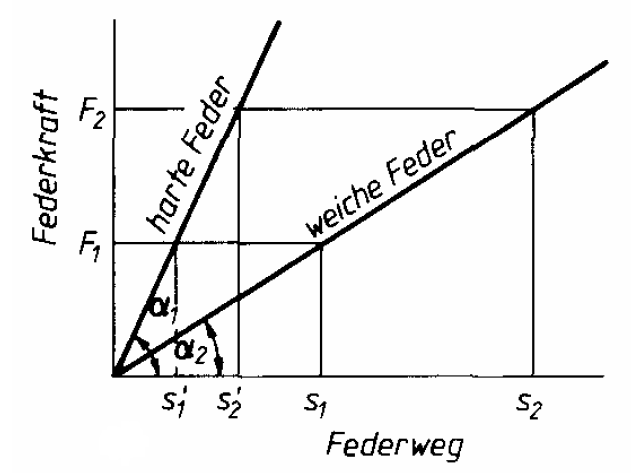
\includegraphics[width=0.52\textwidth]
{Pictures/Federrate.png}}
\subfigure[Federungsarbeit mit Reibungs-Hysterese\citep{Wittel2011}]
{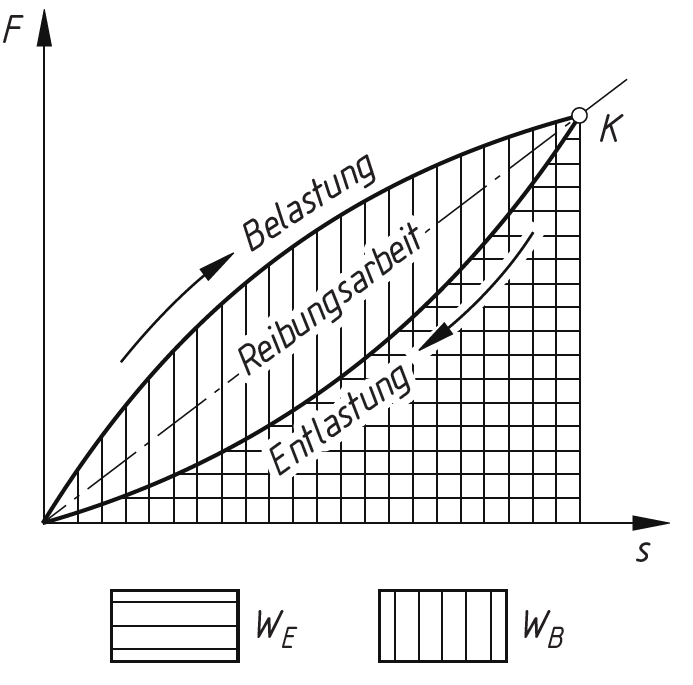
\includegraphics[width=0.4\textwidth]
{Pictures/Federwirkungsgrad.png}}
\caption{Federrate und -wirkungsgrad}
\label{fig:Federrate und -wirkungsgrad}
\end{figure}


Die Biegespannung $\sigma_b$ ist das Verhältnis von der Feder aufzunehmendes Biegemoment $M$ zum Widerstandsmoment $W$. Die Formel für die Biegespannung lautet:

\begin{equation}
\sigma_b = \frac{M}{W}= \frac{6 F l}{b h^2}.
\label{eq:Biegespannung}
\end{equation}

Für rechteckige Blattfeder ergibt sich für den Federweg $s$ am Ende der Feder zu: 

\begin{equation}
s = 4 \frac{l^3}{b h^3} \frac{F}{E}.
\label{eq:Federweg}
\end{equation}

Hierbei ist $E$ das Elastizitätsmodul des verwendeten Werkstoffes. 

Der Federwirkungsgrad jeder realen Feder ist kleiner als 1. Innere und äußere Reibung führen dazu, dass die zur Belastung aufzuwendende Arbeit $W_B$ größer ist als die Arbeit zur Entlastung $W_E$ der Feder, siehe Abbild \ref{fig:Federrate und -wirkungsgrad}(b). Die Formel für $\eta_F$ lautet:

\begin{equation}
\eta_F = \frac{W_E}{W_B}.
\label{eq:}
\end{equation}

Die Auslegung für die verwendete Feder erfolgt im Abschnitt \ref{sec:Waegesystem}. Für weitere Literatur zum Thema Federn wird auf die Litatur \citep{Wittel2011} und \citep{Ettemeyer2007} verwiesen. 


\chapter{Stand der Technik}
\label{cha:Stand der Technik}

In diesem Kapitel werden alle für die Masterarbeit relevanten theoretischen Grundlagen erläutert. 
Zu erst wird in \ref{sec:Kaeltetechnik} die Thermodynamik der Kältetechnik betrachtet. 

\section{Kältetechnik}
\label{sec:Kaeltetechnik}

Die Kältetechnik wird in verschiedensten Einsatzgebieten eingesetzt, um Kälte zu erzeugen bzw. einem definierten Raum Energie in Form von Wärme zu entziehen. 

Das Konservieren von Lebensmittel ist  der ursprüngliche Hauptzwece der Kältetechnik und ist auch heute noch aktuell. Bereits 3000 Jahre v. Chr. nutzten die Ägypter und Mesopotamier Natureis, um ihre Nahrungsmittel länger haltbar zu machen.\citep{Danfoss2006}

Im Jahre 1834 meldete der US-Amerikaner Jacob Perkins sein Patent zum Thema Kältetechnik in England an. Das Patent beschreibt eine Kaltdampfmaschine in einem geschlossenen Kreislauf mit dem feuergefährlichen Äthyläther als Kältemittel.\citep{Siemens2007}

Carl von Linde baute nach konstruktiven Verbesserungen der Kaltdampfmaschine und Verwendung von Ammoniak als Kältemittel im Jahre 1876 die erste praxistaugliche Kälteanlage. Die ersten Anlagen wurden durch die Maschinenfabrik Augsburg-Nürnberg gebaut und an Brauereien sowie später auch an die Schifffahrt vertrieben.

Mit steigender Bedeutung von Elektrizität als Energieträger nach dem 1.Weltkrieg nahm auch die Entwicklung und der Bedarf an Kälteanlagen zu. Im Jahre 1920 startet die Firma General Electric mit der Serienherstellung von Haushaltkühlschränken mit Hermetik-Verdichtern.

Das vielseitige Gebiet der Kältetechnik umfasst alle Technologien, die zur Bereitstellung von Kälteenergie dienen. Sie unterscheiden sich in der benötigten zuzuführenden Energien, Einsatzbereich und eingesetzten Kältemitteln.  Zu den wichtigsten und heute meist verwendeten Technologien gehören folgende Technologien

\begin{itemize}

\item Kompressions-Kälteprozess: \textit{Prozess wird angetrieben durch Zufuhr mechanischer Energie}
\item Sorptions-Kälteprozess: \textit{Prozess wird angetrieben durch Zufuhr von Wärmeenergie}
\item Linde-Verfahren.

\end{itemize}

Weitere nicht so weitverbreitete Technologien der Kältetechnik, jedoch technisch interessante Verfahren  sind zB. das  \textit{Wirbelrohr},  \textit{Magnetische Kühlung} oder das Kühlen mittels einem Peltier-Element. Diese Verfahren werden meist nur unter hohem Energieverbrauch in Sonderfällen angewandt. \citep{Grote2014}

Da sich diese Masterarbeit mit dem Aufbau eines Prüfstandes zur Untersuchung von Abtaumethoden einer Kompressionskälteanlage beschäftigt, wird in den folgenden Kapitel ausschließlich auf diese Technologie eingegangen. Für weitere Informationen bezüglich der anderen Technologien sei an dieser Stelle auf die Literatur \citep{Baehr2013}, \citep{Grote2014} und \citep{Grote2014} verwiesen.


\subsection{Kaltdampf-Kälteprozess}
\label{subsec:Kaltdampf-Kälteprozess}

In diesem Abschnitt wird die Thermodynamik des Kaltdampf-Kälteprozesses näher erläutert. Der Kaltdampf-Kälteprozess ist ein linksläufiger \textit{Clausius-Rankine-Kreisprozess}. Die Zustandspunkte des verwendeten Kältemittels im ln p,h Diagramm sind in Abbildung \ref{fig:Schema p-h-Diagramm} dargestellt. 

\begin{figure}[htb]
\centering		
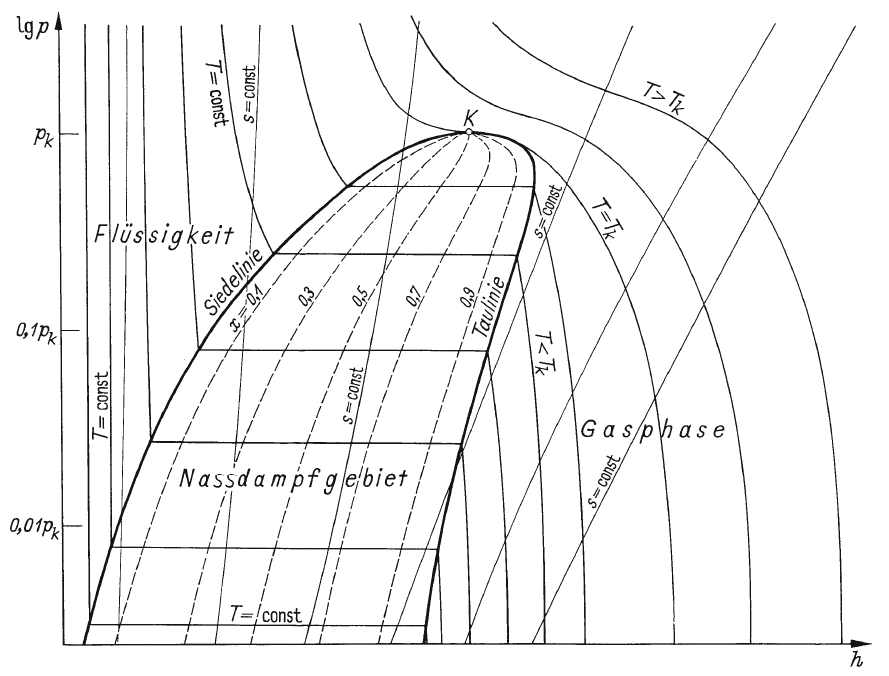
\includegraphics[width=0.75\textwidth]{Pictures/log_p_h_Beahr_Schema.png}
\caption{ln p,h-Diagramm von einem reinen Fluid  \citep{Baehr2013}}
\label{fig:Schema p-h-Diagramm}
\end{figure}

Das halb-logarithmische Diagramm ist ein vielgebrauchtes und hilfreiches Mittel in der Kältetechnik-Branche. 
\footnote{Das Zustandsdiagram wurde vom deutschen Ingenier Richard Mollier (863-1935) im Jahre 1924 erstmalig vorgestellt.} 
Im Diagramm \ref{fig:Schema p-h-Diagramm} ist der Druck logarithmisch auf der y-Achse und die spezifische Enthalpie $h$ auf der x-Achse eingetragen. Die Siedelinie ist durch $x = 0$ und die Taulinie durch $x = 1$. Zwischen $0\leqq x\leqq 1$ befindet sich das Nassdampfgebiet. Es liegt ein Gemisch aus gasförmigen und flüssigem Kältemittel vor. Der Anteil des Gases im Nassdampfgebiet wird durch $x$ ausgedrückt, $1-x$ den Anteil der Flüssigkeit.


In dem Diagramm \ref{fig:Komponeneten und p-h-Diagramm} sind alle Zustandspunkte bei einem Durchlauf des Kältekreislaufes abgebildet.Innerhalb des Nassdampfgebietes verläuft in einem idealen Kältekreislauf, eine Zustandsänderung \textit{isotherm} und \textit{isobar} ab. Wärmezu- oder abfuhr führt nicht zu einer Erhöhung der Temperatur, sondern zu einer Veränderung vom Gas- bzw. Flüssigkeitsanteil. Es wird von einer \textit{latenten}, also nicht fühlbaren,  Wärmeänderung geredet. Um einen Tropfen flüssigen Wasser, dessen Zustand sich auf der Siedelinie befindet, in einen gasförmigigen Zustand, sprich $x=1$ zu überführen, muss ihm die spezifische Verdampfungsenthalpie $\Delta h$ zugeführt werden. Verläuft die Zustandsänderung entgegengesetzt kondensiert der Tropfen und gibt die Verdampfungsenthalpie $\Delta h$ an seine Umgebung ab. 
Außerhalb des Nassdampfgebietes führt eine Wärmezu- oder abfuhr zu einer Veränderung der Temperatur. Die Wärmeänderung ist \textit{sensibel}. 

\begin{figure}[htb]
\centering		
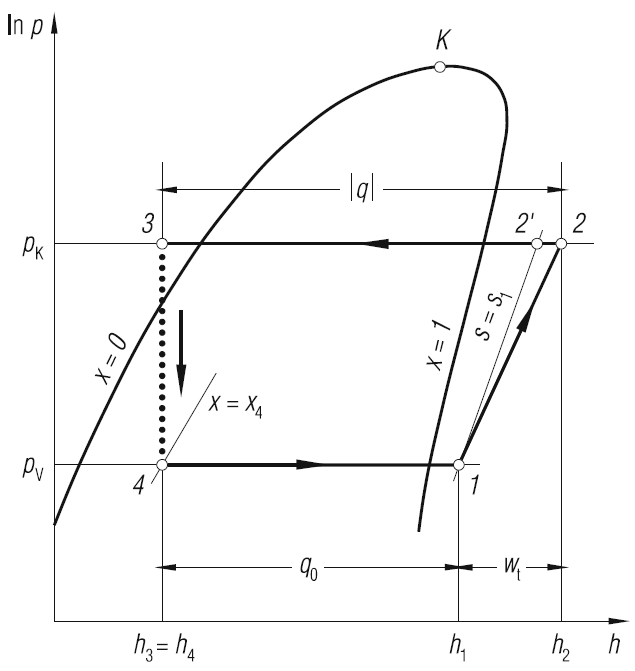
\includegraphics[width=0.6\textwidth]{Pictures/log_p_h_Beahr.png}
\caption{Kreisprozess im ln p,h-Diagramm \citep{Baehr2013}}
\label{fig:Komponeneten und p-h-Diagramm}
\end{figure}


In einem  Kaltdampfprozess, sprich ohne Verluste durch Reibung, finden folgende vier Teilprozesse statt:

\begin{itemize}
\item[1 $\longrightarrow$ 2] Kompression des dampfförmigen Kältemittels unter der Zuführung von elektrischer Leistung $P_{KM}$
\item[2 $\longrightarrow$ 3] Abkühlung, Kondensation und Unterkühlung des Kältemittels unter der Abgabe der Wärmeenergie $\dot{Q}$ über den Verflüssiger an die Umgebung
\item[3 $\longrightarrow$ 4] Entspannung des flüssigen Kältemittels durch das Drosselventil; teilweise setzt die Verdampfung des Fluids ein 
\item[4 $\longrightarrow$ 1] Verdampfung des noch flüssigen Kältemittels auf niedrigem Druckniveau unter der Aufnahme des Wärmestromes $\dot{Q_0}$ aus dem Kühlraum
\end{itemize}

Der Prozess findet auf zwei Durckniveaus statt: dem Verdampfungsdruck $p_V$ und dem Kondensationsdruck $p_K$. Die Verflüssigung des Kältemittels findet auf hohem Druckniveau und die Verdampfung auf niedrigem Druck statt. Die höchste Temperatur wird nach der Kompression am Zustandspunkt 2 erreicht; er befindet sich im Überhitzen- und Hochdruckbereich. Die niedrigste Temperatur ist kurz nach dem Dosselventil und vor dem Verdampfer am Punkt 4. auf niedrigem Druckniveau. 

Nach dem Anwenden des 1. Hauptsatzes der Thermodynamik, die Erhaltung der Energie in einem System, auf den Kältekreislauf folgt die Gleichung :

 \begin{equation}
 	|\dot{Q}|  = \dot{Q_0} +  P_{KM}.
 	\label{eq:Energiebilanz}
 \end{equation}
 
Die elektrische Antriebsleistung der Kältemaschine ist die aufgenommene elektrische Leistung durch den Kompressor zwischen den Zustandspunkten 1  und 2. Sie ergibt sich zu:

\begin{equation}
P_{KM} = \dot{m}~ w_t= \dot{m}~ (h_2 - h_1) = \frac{\dot{m} }{\eta_{sV}} (h_{2'}- h_1).
\label{eq:Antriebsleistung}
\end{equation}

Hierbei ist $\eta_{sV}$ der isentrope Wirkungsgrad des Kompressors. Der isentrope Wirkungsgrad setzt den realen Kältekreislauf in ein Verhältnis zum idealen Kältekreislauf. Die Überhitzung des Gases am Austritt des Kompressors ist höher als die Überhitzung nach einer isentropen Verdichtung. Daraus folgt eine höhere Energieaufnahme durch den Kompressor und ein höherer Wärmestrom $\dot{Q}$, der über den Verflüssiger an die Umgebung abgegeben werden muss. Der isentrope Wirkungsgrad ist definiert über 

\begin{equation}
\eta_{sV}:= \frac{h_{2'}- h_{1}}{h_2 - h_1}.
\label{eq:Antriebsleistung}
\end{equation}


Der Wärmestrom $\dot{Q}$ wird über den Verflüssiger zwischen den Zuständen 2 und 3 abgeführt. Die Formel von  $\dot{Q}$ lautet: 

\begin{equation}
	\dot{Q} = \dot{m}~q_0 = \dot{m}~ (h_3 - h_2)< 0.
	\label{eq:Wärmestrom}
\end{equation}

Der Wärmestrom $\dot{Q}$ ist immer kleiner als Null; er wird dem Kreislauf folglich entzogen.  
 
Über ein Drosselorgan wird das Kältemittel vom hohen Druckniveau auf das niedrigere Druckniveau entspannt. Der Teilprozess findet zwischen den Zustandspunkten 3 und 4 statt und wird als $isenthalp$ angenommen.  
 
Die Kälteleistung $\dot{Q_0}$, sprich den aus dem Kühlraum zu entnehmender Wärmestrom, ergibt sich aus dem Kältemittel-Massenstrom $\dot{m}$ und den spezifischen Enthalpien der Zustände 4 und 1 :

\begin{equation}
	\dot{Q_0} = \dot{m}~ q_0 = \dot{m}~ (h_1 - h_4).
	\label{eq:Kälteleistung}
\end{equation}




Die Bewertung einer Kälteanlage erfolgt durch die Leistungszahl $\epsilon_{KM}$: 

\begin{equation}
	\epsilon_{KM} := \frac{Kälteleistung}{Antriebsleistung} =\frac{\dot{Q_0}}{P_{KM}}.
	\label{eq:Leistungszahl}
\end{equation}

Ziel bei der Auslegung und dem Betrieb einer Kältemaschine ist eine möglichst große Leistungszahl zu erlangen. Damit $\epsilon_{KM}$ groß wird, muss die Kälteleistung $\dot{Q_0}$ groß werden und die aufgewandte Verdichterleistung $P_{KM}$ klein werden. 


\subsection{Komponenten eines Kaltdampfprozesses}
\label{subsec:Komponenten eines Kaltdampfprozesses}

Die Komponenten für einen einfachen Kaltdampfprozess  besteht aus vier Komponenten:

\begin{itemize}
\item der Kompressor
\item der Verflüssiger 
\item das Drosselvenil Expansionsventil
\item der Verdampfer. 
\end{itemize}

In Abbildung \ref{fig:einfacher Kältekreislauf} sind die vier Komponenten mit ihren Zustandspunkten dargestellt.

\begin{figure}[htb]
\centering		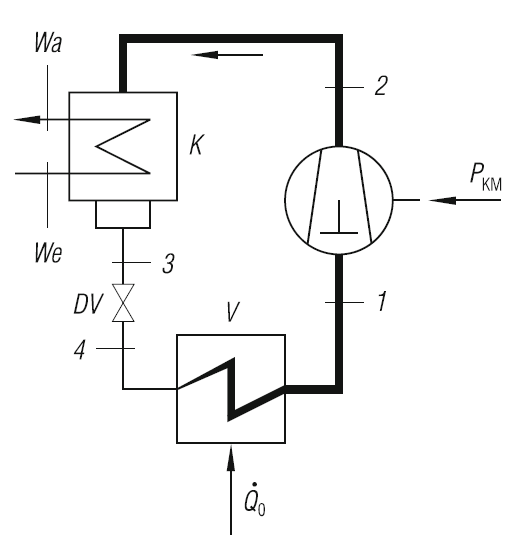
\includegraphics[width=0.50\textwidth]{Pictures/Kaltekreislauf_beahr.png}
\caption{Einfacher Kältekreislauf \citep{Baehr2013}}
\label{fig:einfacher Kältekreislauf}
\end{figure}

\subsubsection*{Der Kompressor}
Der Kompressor bildet das Herzstück der Kälteanlage. Er verdichtet das gasförmige Kältemittel von niedrigem Druck auf ein höheres Druckniveau. Um diese Arbeit zu verrichten, wird der Verdichter mit elektrischer Energie versorgt. Der Kompressor gibt es in verschiedenen Bauvarianten. Die zwei wichtigsten Bauvarianten sind der \textit{Hubkolbenverdichter} und der \textit{Rotationskolbenverdichter}. Die Baugruppen der Verdichter werden in offene, halbhermetische und vollhermetische Verdichter unterschieden. Schrauben-,Scroll- sowie Turboverdichter sind Bauarten der \textit{Rotationskolbenverdichter}. 



Ein wichtiges Kriterium bei Verdichtern ist das Druckverhältnis von Ansaugdruck, vor der Kompression, und dem Ausgangsdruck. Das Druckverhältnis $\pi$ ist definiert als:



\begin{equation}
\pi := \frac{p_{aus}}{p_{ein}}.
\label{Druckverhältnis}
\end{equation}

\subsubsection*{Der Verflüssiger}

Dem Kältemittel wird im Verflüssiger auf einem hohen Druckniveau Wärme entzogen. Der Verflüssiger kühlt das überhitzte, gasförmige Kältemittel ab. Beim Austritt aus dem Verflüssiger ist das Kältemittel meist vollständig kondensiert. 
Um einen Wärmeentzug zu bewerkstelligen gibt es drei Bautypen:

\begin{itemize}
\item Wassergekühlte Verflüssiger
\item Luftgekühlte Verflüssiger
\item Verdunstungsverflüsssiger
\end{itemize}

Wassergekühlte Verflüssiger können, aufgrund der besseren Wäärmeübertragung verglichen zu Luft, sehr kompakt gebaut werden. Eine typische Bauform ist das \textit{Bündelrohrverflüssiger}.
In der Praxis werden am häufigsten luftgekühlte Verflüssiger eingesetzt. Um die gleiche Kühlleistung wie ein wassergekühlter Verflüssiger zu erreichen, werden Lamellen und Ventilatoren eingesetzt. Die Lamellen vergrößern die Fläche für die Wärmeübertragung mit der Luft. Ventilatoren ermöglichen durch einen höheren Luftdurchsatz und der daraus resultierendem höhere Wärmeübertragung eine größere Kühlleistung und eine kompaktere Bauform der Wärmeübertragers. Diese Variante hat den Vorteil, dass die einen wartungsfreien Betrieb  sowie eine einfache Reinigung ermöglicht.


\subsubsection*{Das Expansionsventil}

Das Expansionsventil versorgt den Verdampfer mit dem nötigen Kältemittel-Massenstrom. Die Zuführung des Kältemittels erfolgt über eine Druckdifferenz. Durch eine lokale Verengung des Strömungquerschnitts, verringet sich der Druck des durchfließenden Kältemittels. Das Kältemittel vergrößert sein Volumen und es kommt zur Expansion. Die Druckreduzierung erfolgt ohne zusätzliche Arbeit. Im idealen Fall wird bei diesem Prozess auch keine Wärme abgefuhrt; der Prozess ist \textit{isenthalb}. 
Das Expansionsventil trennt zusammen mit dem Kompressor die zwei Druckseiten des Kältekreislaufes. Es gibt Expansionsventile sowohl als regelbare und nicht regelbare Ausführungen. Bei kleineren Anlagen erfolgt die Expansion ungeregelt zum Beispiel durch Kapillarrohre. Geregelte Expansionsventile werden in mittleren und großen Kälteanlagen eingesetzt. Die Regelung erfolgt durch die Querschnittsänderung und dem damit einhergehendem Druckabfall.  

\subsubsection*{Der Verdampfer}

In dem Verdampfer wird das Kältemittel eingespritzt. Das Kältemittel verdampft und entzieht seiner Umgebung dabei Wärme. Aufgrund der vielfältigen Anforderungen an Verdampfer, gibt es eine Vielzahl an Bauarten für Verdampfer. Mögliche Bauarten sind 

\begin{itemize}
\item Glattrohrverdampfer
\item Beripptes Verdampferregister
\item Rippenrohrverdampfer
\end{itemize}

Um eine möglichst große Kälteleistung zu ermöglichen, werden wie beim Verflüssiger auch, Ventilatoren eingesetzt. Die Ventilatoren erzwingen einen Luftstrom durch den Verdampfer und erhöhen damit die Wärmeübertragung zwischen der Luft und den Verdampferrohren. 



\section{Thermodynamik der feuchten Luft}
\label{sec:Thermodynamik der feuchten Luft}

Ein Verdampfer hat die Aufgabe einer Umgebung Energie in Form von Wärme zu entziehen. Hierfür wird in einem Wärmeübetrager flüssiges Kältemittel verdampft. Das verdampfende Kältemittel kühlt zunächst den Wärmeübertrager, danach wird über die Wärmeübertrager-Lamellen der vorbeiströmende Luft Wärme entzogen. 

Bei dem Kühlprozess durch einen Verdampfer kommt es zwischen dem Wärmeübertrager und der feuchten Luft verschiedenen thermodynamischen Phänomenen. Die auftretenden Phänomene lassen sich in folgende Gruppen einordnen:

\begin{itemize}
\item	Abkühlung der feuchter Luft 
\item 	Wassertropfenbildung auf Lamellenoberfläche 
\item	Kristallbildung auf Lamellenoberfläche.
\end{itemize}

In den nachfolgenden Abschnitten \ref{subsec:Feuchte Luft} und \ref{subsec:Reifbildung} werden die Phänomene kurz erklärt.

\subsection{Feuchte Luft}
\label{subsec:Feuchte Luft}

\begin{figure}[htb]
\centering		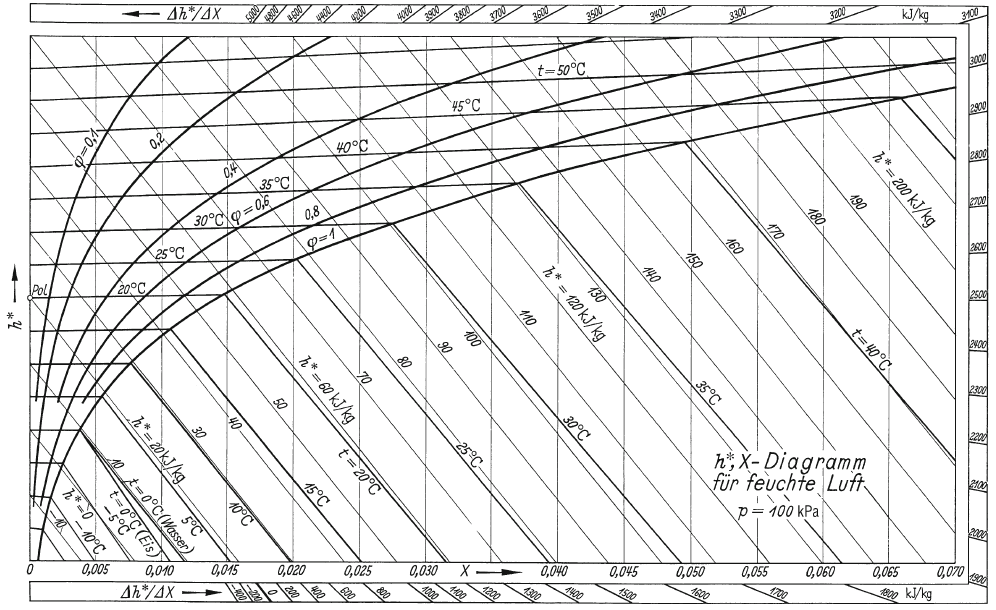
\includegraphics[width=0.85\textwidth]{Pictures/h_x_Diagramm_Beahr.png}
\caption{$h^*$, $X$- Diagramm für feuchte Luft bei einem Gesamtdruck $p= $ 100 kPa \citep{Baehr2013}}
\label{fig:h_x_diagramm}
\end{figure}


Bei dem Wärmeentzug durch den Verdampfer wird  zunächst die noch nicht gesättigte feuchte Luft abgekühlt. Luft besitzt die Eigenschaft eine bestimmte Menge Wasser aufnehmen zu können. Warme Luft kann mehr Wasser aufnehmen als kalte Luft. Das Verhältnis von der aufgenommene Masse Wasser zur Masse Luft ist definiert als Beladung: 

\begin{equation}
X = \frac{m_W}{m_L}.
\label{eq:Beladung}
\end{equation}

In dieser Formel bezieht sich $m_W$ auf gasförmige, flüssige oder feste Form von Wasser und $m_L$ auf die Masse der trockenen Luft.  $X$ kann werden zwischen 0 für trockene Luft und $\infty$ für reines Wasser annehmen. In der Regel bleibt $X$ jedoch kleiner als 0,1. 

Die absolute Feuchte ist definiert als das Verhältnis von Masse des Wasserdampfers $m_W$ zum eingenommen Volumen $V$ der feuchten Luft. Die Formel lautet: 

\begin{equation}
\varrho := \frac{m_W}{V} = \frac{p_w}{R_W T}.
\label{eq:Absolute Feuchte}
\end{equation}


Die relativen Feuchte $\varphi$ ist das Verhältnis der absoluten Feuchte im Verhälnis zur Maximalwert oder Sättigungswert der absoluten Feuchte: 

\begin{equation}
 \varphi := \frac{\varrho}{\varrho_W^s}.
 \label{eq:Rel Feuchte}
\end{equation}

Wird nun in die Gleichung \ref{eq:Beladung} die relative Feuchte aus Gleichung \ref{eq:Rel Feuchte} eingesetzt, ergibt sich eine weitere Formel für die Beladung $X$. 

\begin{equation}
X = \frac{m_W}{m_L} = 0,622 \frac{p_{W}^s}{p/\varphi - p_{W}^s}.
\label{eq:Beladung 2}
\end{equation}

Hierbei ist $p_{W}^s$ der Partialdruck des Sättigungspunktes.
Betrachtet man nur die Wasserdampfbeladung der Luft, so lässt sich feststellen, dass die maximale Menge an aufzunehmenden Wasser einen Grenzwert hat. Dieser Grenzwert wird Sättigungswert der Wasserdampfbeladung genannt und ist eine Funktion abhängig von der Temperatur und dem Druck.  Sie berechnet sich nach dem Gesetz von Dalton zu :

\begin{equation}
 X_s (T,p) = 0,622 \frac{p_{W}^s}{p - p_{W}^s}.
 \label{eq:Sättigungsbeladung}
\end{equation}

Bei der Abkühlung von feuchter Luft kann der Fall eintreten, dass $X > X_s$ ist. Sprich die Beladung der trockenen Luft ist größer als das alles im Wasserdampf aufgenommen werden kann. Der erste Tropfen Kondensat bildet sich und Wasser fällt aus. Es ergibt sich eine Kondesationsmenge von:

\begin{equation}
\Delta X m_L = (X - X_s)m_L.
\label{eq:Delta_X}
\end{equation}

Die Wassermenge $X_s m_L$ ist gasförmig von der trockenen Luft gespeichert. Die Kondensationsmenge $\Delta X m_L$ setzt sich nun an Keimpunkten in der Umgebung ab oder wird als Nebel aus der Gasphase ausgeschieden. Keimzellen für Wassertropfen können zum Beispiel Verunreinigungen oder raue Oberflächen sein. Das höchste treibende Potential für eine solche Keimzelle hat der kälteste Punkt im System. In unserem Anwendungsfall ist das der Wärmeübertrager des Verdampfer. Da der Verdampfer zur Bereitstellung der Kälteleistung und einer funktionierenden Wärmeübertragung stets eine Temperaturdifferenz zwischen dem Kältemittel und der vorbei strömenden Luft  bereitstellt,  bilden sich hier die ersten Tropfen. Je nach ursprünglicher Beladung der Luft bilden sich die Tropfen eher am Anfang oder Ende des Wärmeübertrager. War die feuchte Luft schon vor dem Eintritt in den Wärmeübertrager bereits stark gesättigt, bilden sich Tropfen am Eingang der Lamellen. 
\citep{Baehr2013}


\subsection{Reif- und Eisbildung}
\label{subsec:Reifbildung}

Liegt die Oberflächentemperatur auf dem Wärmeübertrager des Verdampfers nicht nur unter dem Taupunktpunkt der feuchten Luft sondern auch unter dem Gefrierpunkt, kann es zum Gefrieren der kondensierten Tropfen und/oder zur Desublimation von Wasserpartikel auf der Oberfläche kommen. Dieser Abschnitt soll einen Überblick über diese zwei thermodynamischen Phänome geben. Da in dieser Arbeit nicht der Reifbildungsprozess im Hauptfokus steht, sondern  der technische Aspekt der Abtauung, wird der Eisbildungsprozess hier nur kurz erläutert.

In der Literatur gibt es zahlreiche Quellen, die sich mit der Reif- bzw. Eisbildung auseinander setzen. Die Quellen beschreiben den Kristallbildungsprozess sowohl aus der rein theoretisch Sicht als auch simulationsrelevanten und technischen Überlegungen und Untersuchungen. Der scheinbar triviale Prozess von der Bildung eines Eiskristalles auf einer Oberfläche und sein weiteres Wachstumsverhalten ist sehr komplex und Gegenstand zahlreicher aktueller und schon abgeschlossener Forschungsprojekten.

Neben den theoretischen Grundlagen wird in der Arbeit von \textsc{\citeauthor{Schydlo2010}} ein Simulationsmodell für den Reifbildungs- und Abtauprozess auf einem Rohr entwickelt. Zudem sind bisherigen Arbeiten zu der Thematik in \citep{Schydlo2010} aufgelistet und zusammengefasst. 
Praktische Untersuchungen sowie Versuchsaufbauten zum Thema der Vereisung von Luftkühler werden in \textsc{\citeauthor{Sahinagic2004}} und \textsc{\citeauthor{Kosowski2009}} beschrieben. In den Arbeiten wurden die Vereisungs- und innovative Abtauungsprozesse von einer CO$_2$-Wärmepumpe, die zur Heizung von Passivhäuser eingesetzt wird, untersucht.   



Es gibt zahlreiche Einflussgrößen die auf den Prozess und die Form des Eiskristalls und späteren Reif einwirkten. 
  Die wichtigsten Einflussgrößen sind die Luftgeschwindigkeit, die Lufttemperatur, die Luftfeuchte, die Oberflächentemperatur und die Zeit. Um eine den Reif charakterisieren zu können, werden folgende Größen zur Hilfe genommen die Reifdicke, die Reifdichte, die Porösität und die Wärmeleitfähigkeit. 

In der Arbeit von \textsc{\citeauthor{Hayashi1977}} aus dem Jahre 1977 wird der Eiskristallwachstum in drei Phasen unterteilt:

\begin{enumerate}
\item Eindimensionales Kristallwachstum
\item Reifschichtwachstumsphase 
\item Vergletscherung.
\end{enumerate}


\begin{figure}[htb]
\centering		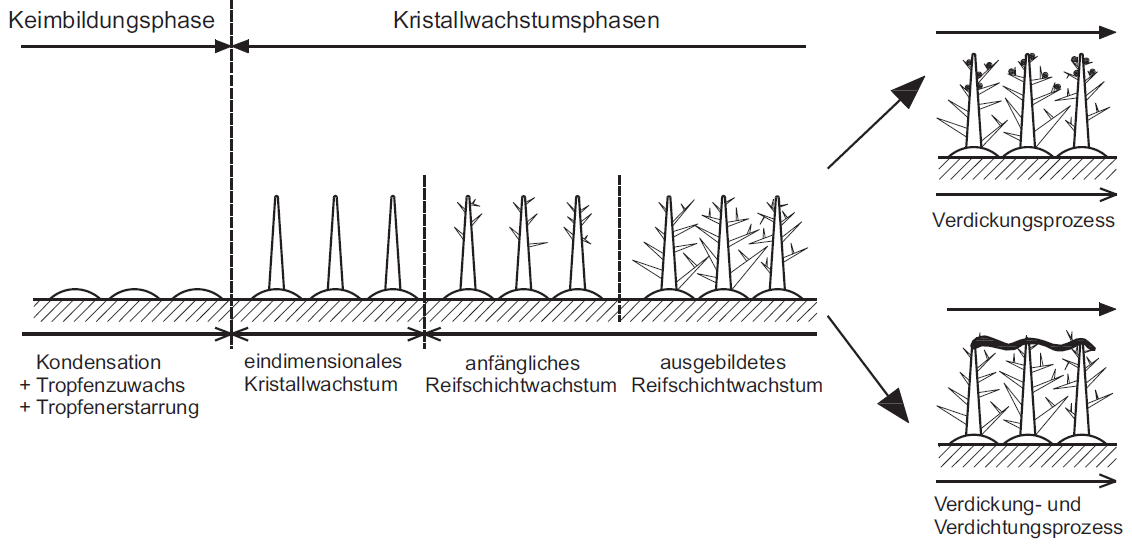
\includegraphics[width=0.85\textwidth]{Pictures/Reifbildungsphasen_Schydlo.png}
\caption{Kristallwachstum auf einer ebenen Oberfläche \citep{Schydlo2010}}
\label{fig:Kristallwachstum}
\end{figure}


In Abbildung \ref{fig:Kristallwachstum} sind die drei Kristallwachstums-Phasen nach \textsc{\citeauthor{Hayashi1977}} sowie die vorhergehende Keimbildungsphase, , eingeführt in \citep{Sahinagic2004}, dargestellt. 

\subsection*{Keimbildungsphase}

In der Keimbildungsphase bilden sich zunächst Wassertropfen auf der Lamellenoberfläche, die trotz Temperaturen kleiner als der Gefrierpunkt nicht erstarren, sondern wachsen zu größeren Tropfen an. Je kleiner die Unterkühlung desto größer werden die Tropfen bevor sie erstarren und in die erste Kristallwachstumsphase übergehen. 

\subsection*{Eindimensionales Kristallwachstum}
Die erste Phase ist gekennzeichnet durch Kristallwachstum senkrecht zur Oberfläche und mit einheitlicher Wachstumsgeschwindigkeit. Dies führt zu einer erhöhten Rauigkeit aufgrund der sich stetig vermehrenden Kristalle. 

\subsection*{Reifschichtwachstumsphase}
In der zweiten Phase beginnt das dreidimensionale Wachstum. Die Kristalle fangen an sich miteinander zu verästeln. Ein poröses Kristallgitter entsteht. Aufgrund des  Wärmeleitwiderstandes, der mit der Reifdicke steigt, erhöht sich die Oberflächentemperatur der Reifschicht. Desweiteren kommt es zu einem Massenstrom innerhalb der Reifschicht, ausgelöst durch Diffusion. Die Diffusion rührt aus  den  Konzentrationsunterschiede zwischen der Lamelle und der Reifoberfläche. Der Wassermassenstrom läuft in das poröse Kristallgitter und gefriert dort in Nähe der Lamelle. Die Dichte der Reifschicht steigt und mit ihr der Wärmewiderstand. Dies führt zu einer Erhöhung der Oberflächentemperatur der Reifschicht und schließlich zur Überschreitung des Gefrierpunktes von Eis. Die Spitzen des Kristalle schmelzen und es bildet sich Kondensat. Die dritte Wachstumsphase beginnt. 

\subsection*{Vergletscherung}

Das flüssige Wasser läuft aufgrund der Kapillarwirkung der Kristalle in die Zwischenräume des Kristalgitters und gefriert dort wieder. Die Kristallgitter werden dichter und kompakter. Dies führt zur Steigerung der Wärmeleitfähigkeit der Reifschicht. Es wird von einer Vergletscherung gesprochen. Die Oberflächentemperatur der Reifschicht sinkt erneut und fällt erneut unter den Gefrierpunkt. Nun kann die feuchte Luft erneut an der Oberfläche des Reifs desublimieren. Der Prozess wiederholt sich solange bis das Eis so kompakt ist, dass kein weiteres Kondensat mehr in die Reifschicht eindringen kann. 
    





\section{Morphologie von Eiskristallen}
\label{sec:Morphologie}







\chapter{Versuchsaufbau}
\label{cha: Versuchsaufbau}

Dieses Kapitel beschreibt den Aufbau des gesamten Versuchsstandes. Zunächst wird in Abschnitt \ref{sec:Kältetechnischer Aufbau} der Aufbau und die Funktionsweise der Kälteanlage und der Klimakammer erläutert. Im Weiteren wird in Abschnitt \ref{sec:Waegesystem} auf das Konzept und Aufbau des Wägesystems eingegangen. 
Der elektrische Aufbau des Versuchsstandes wird in Abschnitt \ref{sec:Elektrischer Aufbau} näher erläutert, um im darauf folgenden Abschnitt \ref{sec:Informationstechnischer Aufbau} den informationstechnischen Aufbau zu erklären. 




\input{Chapters/Versuchsaufbau/Kältetechnischer_Aufbau.tex}

\input{Chapters/Versuchsaufbau/Wägesystem.tex}

\section{Elektrischer Aufbau}
\label{sec:Elektrischer Aufbau}
Im Zuge der Arbeit wird die KA, die zuvor nur manuell betrieben werden konnte, vollständig auf eine SPS umgebaut. Zu berücksichtigen ist dabei die Hardware-Schaltschrank-Architektur des manuellen Betriebes. Für den manuellen Betrieb hatte die KA zwei Schaltschränke zur Versorgung der Komponenten mit der Hilfsenergie, sowie zur Ansteuerung der Magnetventile und des Vierwegeventils.

Um den Umbau auf eine SPS vollziehen zu können, ist es nötig, das elektrische Konzept für den manuellen Betrieb nachzuvollziehen, um  gleiche Funktionalität und Sicherheit der KA im SPS-Betrieb gewährleisten zu können. Es wird versucht einen möglichst großen Anteil der Komponenten des manuellen Betriebes  in das neue elektrische Konzept der SPS einzubinden. Nach dem Umbau wird die KA ausschließlich über die SPS bedienbar sein. Der manuelle Betrieb über Schalter wird nicht mehr möglich sein, jedoch wird es einen \textit{Manuellen-Modus}im späteren informationstechnischen Konzept geben, siehe Abschnitt \ref{sec:Informationstechnischer Aufbau}.

Das elektrische Konzept umfasst folgende Teilaspekte bzw. -funktionen:

\begin{itemize}
\item Auslesen von Sensoren
\item Stellen von Aktoren 
\item Versorgung der Aktoren/Sensoren mit Hilfsenergie.
\end{itemize}

Das \textit{Auslesen von Sensoren} umfasst das Auslesen von Temperatur, Druck, Massenstrom, Gewichte der Waagen sowie die Ventilöffnungen der Expansionsventile. Das \textit{Stellen von Aktoren} besteht aus der Sollwertvorgabe für die Kompressor- und Verflüssigerventilatordrehzahl, elektrische Heizung sowie das An- und Ausschalten der Ventilatoren vom Verdampfer und Abtauverdampfer. Des Weiteren werden Magnet- und Vierwegeventile geschaltet. 
Die \textit{Versorgung der Aktoren/Sensoren mit Hilfsenergie} gewährleistet einen sicheren Betrieb der KA und die Funktionalität der Komponenten.  
%Der Frequenzumformer des Kompressor wurde manuell über ein Touchpad angesprochen. Über das Touchpad wurde der Sollwert des Saugdruckes vorgegeben.  

Das elektrische Konzept sieht eine zentralisierte elektrische Installation vor. Für die KA sind sowohl Analoge Ein- und Ausgangssignale (0..10 V DC, 4..20 mA), Digitale Ausgangssignale (0...24 V DC). Diese Signale werden über maximal 10 m gesendet. Die Verwendung eines Buskopplersystem ist folglich nicht notwendig. Die meisten Signale werden jedoch nur über wenige Meter zu den benachbarten Schaltschränken gesendet. Hierbei ist mit keinen Problemen durch elektromagnetische Störungen zu rechnen. 

Für das Auslesen der Sensoren, die maximal  20 m von dem SPS-Schaltschrank enfernt sind, wird ein Bussysteme (MODBUS RTU) eingesetzt. Dieses Bussystem erlaubt es bis zu 32 Sensoren auf einer Entfernung von theoretisch 1000 m anzuschließen. Im Abschnitt \ref{subsec:Modbus} wird das Protokoll \textit{Modbus RTU} und der elektrische Aufbau des Modbuses erklärt. 
 
Die SPS besteht aus dem CPU-Grundmodul \textit{CX9020} sowie Busklemmen der Fa. Beckhoff. Die Busklemmen sind vom Typ E-Bus, die das firmeneigene Protokoll EtherCAT (Ethernet for Control Automation Technolog) unterstützen.  Das EtherCAT verfügt neben ihrer Echtfähigkeit(1.000 verteilte I/Os in 30 $\mu s$\citep{Beckhoff2016}) auch über die Fähigkeit zur Einbindung von  Standardethernet Komponenten und flexiblen Typologien. Bei einen E-Bus (ELxxxx)wird das Prozessabbild mittels des EtherCAT
Protokolls, das abgeleitet vom Standard Ethernet Protokoll ist, bis an die jeweilige Busklemme übermittelt. Die Busklemme kanndann ihren Wert lesen bzw. schreiben. Dieses Verfahren erlaubt äußerst geringe Zykluszeiten. Abbildung \ref{fig:Beckhoffklemmen} zeigt exemplarisch das Grundmodul CX9020 und eine PT100-Temperatur-Busklemme. Der CX9020 verfügt über einen 1-GHz-CPU und läuft mit dem Betriebssystem Windows CE. Es wird auf einer Hutschiene montiert und erkennt angeschlossene Busklemmen automatisch. 

\begin{figure}[htb]
\centering
\subfigure[Ethernet-Steuerungs-CPU CX9020]
{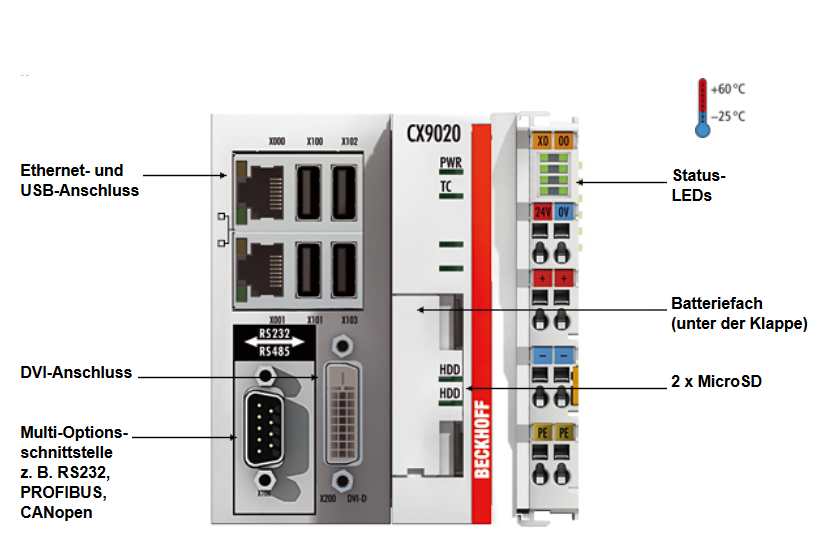
\includegraphics[width=0.52\textwidth]
{Pictures/CX9020.png}}
\subfigure[EL3202: 2-Kanal-Eingangsklemmen für PT100-Temperatursensoren]{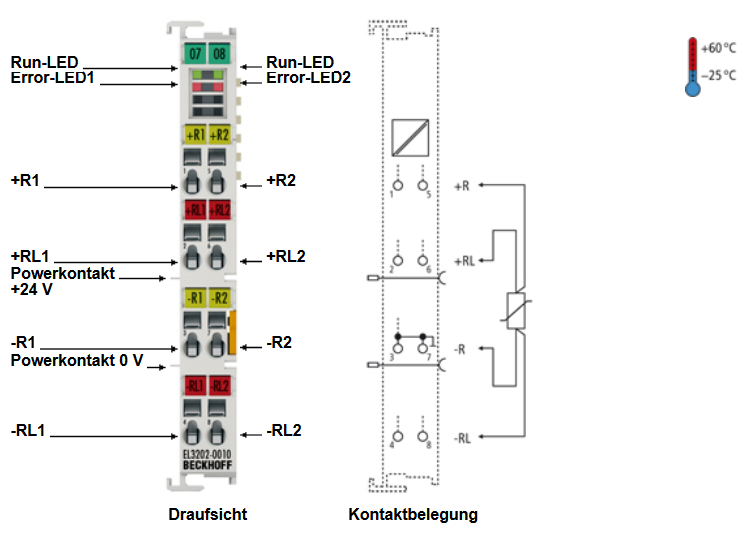
\includegraphics[width=0.42\textwidth]
{Pictures/EL3202.png}}
\caption{SPS-CPU und E-Busklemme der Fa. Beckhoff}
\label{fig:Beckhoffklemmen}
\end{figure}

In Tabelle \ref{tab: Beckhoff-Busklemmen- Übersicht} sind alle verwendeten Klemmen mit Kanalanzahl, Signalart und der eingesetzten Anzahl aufgelistet. 

Der CX-9020 verfügt über zwei RJ45 Anschlüsse für LAN-Schnittstellen. Hier können weitere Buskoppler oder ein PC angeschlossen werden. Buskoppler kommunizieren über EtherCAT  und der PC über TCP/IP mit dem Gerät. Eine der zwei Schnittstellen dient zur Kommunikation mit dem Host-PC. Vier USB-Schnittstellen dienen für einen Anschluss von beispielsweise einer Maus, Tastatur  oder eines Speichermediums. 

\begin{table}[htb]
\centering
\caption{Busklemmen-Übersicht}\vspace{6pt}
\begin{tabular}{p{2cm}p{3.6cm}p{1.4cm}p{2.8cm}p{3.2cm}ccccc}
\hline 
\rule[-1ex]{0pt}{2.5ex} \textbf{Klemmennummer} & \textbf{Typ} & \textbf{Anzahl Kanäle} & \textbf{Signal} & \textbf{Eingesetze Anzahl} \\ 
\hline 
\hline 
\rule[-1ex]{0pt}{2.5ex} EL 4024 & Analog Ausgang & 4 & 4..20 mA & 1 \\ 
\hline 
\rule[-1ex]{0pt}{2.5ex} EL 4008 & Analog Ausgang & 8 & 0..10 V DC & 1 \\ 
\hline 
\rule[-1ex]{0pt}{2.5ex} EL 3202 & Analog Eingang & 2 & Temperatur (°C) & 6 \\ 
\hline 
\rule[-1ex]{0pt}{2.5ex} EL 3054 & Analog Eingang & 4 & 4..20 mA & 1 \\ 
\hline 
\rule[-1ex]{0pt}{2.5ex} EL 2809 & Digital Ausgang & 16 & 24 V DC  & 1 \\ 
\hline 
\rule[-1ex]{0pt}{2.5ex} EL 6021 & Serielle Schnittstelle & 1 &  RS422/RS485 & 1 \\ 
\hline 
\rule[-1ex]{0pt}{2.5ex} EL 9410 & E-Bus Auffrischung & 0 & - & 1 \\ 
\hline 
\rule[-1ex]{0pt}{2.5ex} EL 6002 & Serielle Schnittstellen & 2 & RS232 & 3 \\ 
\hline 
\rule[-1ex]{0pt}{2.5ex} EL 9011 & Endklemme & 0 & - & 1 \\ 
\hline 
\hline 
\end{tabular} 
\label{tab:Klemmenübersicht}
\end{table}



Der CX-9020 wird an ein Trafo von der Fa. Siemens mit 24 V DC versorgt. Über die Kanäle 24 V und 0 V wird der Buskoppler EK 1200 mit Spannung gespeist. Der EK 1200 kommuniziert per E-Bus mit den angeschlossenen Klemmen und versorgt diese über die Powerkontakte mit Spannung.  Der Buskoppler ist in den den CX-9020 integriert. Die EK 1200 stellt eine Stromversorgung von 1860 mA zur Verfügung.  Jede Klemme hat einen Stromverbrauch im Bereich von 50-190 mA. Eine Unterschreitung der 0 mA Grenze ist möglich, kann laut Hersteller jedoch zu Kommunikationsproblemen führen und ist zu vermeiden. Deshalb wird eine E-Bus-Auffrischungsklemme EL 9410 zur Einspeisung weiterer 1860 mA in den E-Bus integriert. 

Jede Klemme verfügt je nach Ausführung über verschiedene Diagnose-LEDs, die Auskunft über korrekten Anschluss, Betriebsstatus oder eventuelle Fehler geben. Die Kommunikation zu den Busklemmen erfolgt über die Kontakte an der Seite (E-Bus). Die Ausführungen der Busklemmen sind sehr vielfältig. Sie unterscheiden sich in der Kanalanzahl, Genauigkeit, Auflösung etc. Abbildung \ref{fig:Beckhoffklemmen} zeigt den CX-9020 und eine EL 3202 für zwei PT100-Temperaturelemente. 

Der Beckhoff-Schaltschrank wird über eine separate Spannungsquelle, getrennt von anderen elektrischen Komponenten,  versorgt. Dies erlaubt ein Betrieb der SPS, zB. fürs Progammieren oder Testen, unabhängig von den anderen Schaltschränken. 

Folgende Komponenten der KA werden elektrisch an die SPS angeschlossen: 
\begin{itemize}
\item	Kompressor-Frequenzregelung mit analogem Ausgangsignal 4..20 mA
\item	Verflüssigungsregelung mit analogem Ausgangsignal  0..20 mA
\item	Elektrische Heizungselemente analogem Ausgangsignal mit 0..10 V
\item	Schaltschütze mit digitalem Ausgangssignal 0..24 V DC für Magnetventile, 4-Wegeventil, Spannungsfreigabe für Verdampfer-Ventilatoren
\item 	Modbus RTU über COM-Schnittstelle und RS-485 Klemme
\item 	PT100- Temperaturelemente 
\end{itemize}

Für die genaue elektrische Installation wird an dieser Stelle an die Handbücher der jeweiligen Komponenten verwiesen. Elektrische Arbeiten über 50 V wurden von der elektrischen Werkstatt des Instituts durchgeführt. \citep{MicroNovaAG2011}

\newpage
\subsection{Modbus RTU}
\label{subsec:Modbus}

Ein Auslesen von Sensoren kann über analoge Ausgangssignale, zB. 4-20 mA oder älter 0-20 mA, geschehen oder über Bussysteme. Beide Varianten sind in der Praxis weit verbreitet. Je nach Menge der Sensoren und Entfernungen zwischen den Sensoren wird sich für eine Variante entschieden. Feldbusse sind nach der Norm IEC 61158 \footnote{\textit{Digital data communication for measurement and control - Fieldbus for use in industrial control systems}} weltweit standardisiert. 

Die Verwendung von Feldbussen hat sowohl Vor- und Nachteile. Die Vorteile sind der geringe Verkabelungsaufwand oder Eigendiagnose durch das System sind möglich. Ein Feldbuss-System bietet eine hohe Flexibilität gegenüber Erweiterungen oder Änderung des Netzwerkes. Eine Festlegung auf Messbereiche der Sensoren ist nicht notwendig. Ein weiterer Vorteil ist die Möglichkeit der Abfrage unterschiedlicher Messwerte, wie zum Beispiel Temperatur und Druck, von einem Sensor. Die hohe Zuverlässigkeit und hohe Kompatibilität von verschiedenen Sensortypen ist ein weiterer großer Vorteil.

Die Nachteile eines Feldbusses sind die komplexere Netzwerkstrukturen und -abläufe. Ein höher qualifiziertes Personal ist eine Voraussetzung für eine erfolgreiche Implementierung eines Feldbuss-Systems. Des Weiteren erfordert eine Abfrage der Sensoren meist eine größere Reaktionszeit. Sensoren mit der entsprechender Feldbustechnik sind häufig teurer als Sensoren, die mit analogen Datenübertragung ausgestattet sind. Eine Beschädigung des Kabels kann in manchen Fällen zu dem Ausfall des kompletten Feldbusses und dessen Sensoren führen. Redundante Netzwerke sind folglich wünschenswert, jedoch nicht immer umsetzbar. 

\begin{figure}[htb]
 \centering		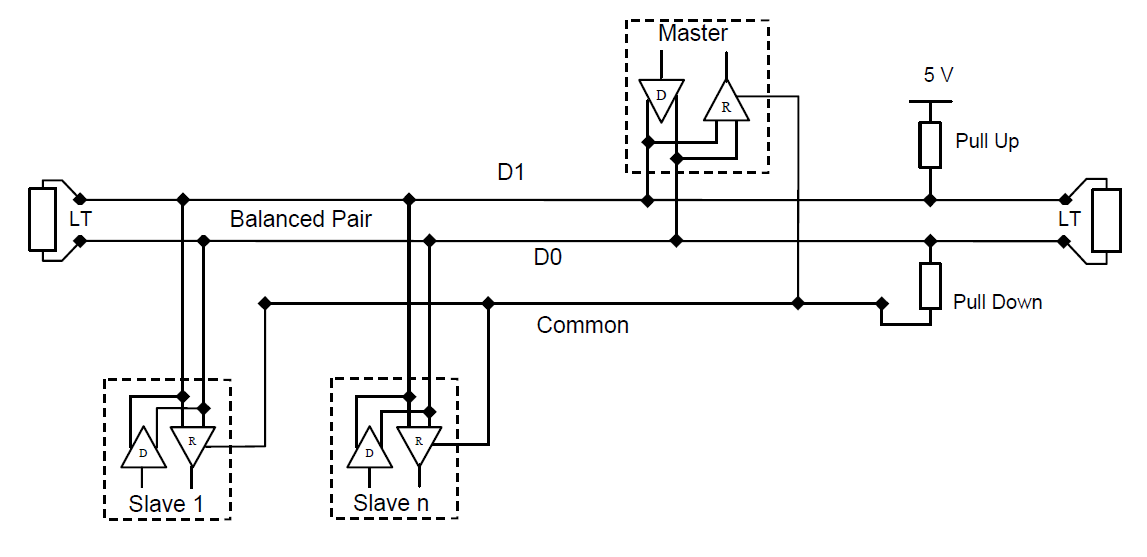
\includegraphics[width=0.94\textwidth]{Pictures/TopologieModbus.png}
 \caption{Zwei-Kabel-Topologie eines MODBUS RTU- Feldbusses \citep{MODBUS.ORG2002}  }
 \label{fig:ZweiKabelModbus}
 \end{figure} 

Feldbusse können mit verschiedenen Netzwerk-Topologien ausgeführt werden. Für den Modbus RTU wird nach \citep{MODBUS.ORG2002} eine Serienschaltung der Hardware-Komponenten (engl. \textit{Daisy Chain}) empfohlen. Die Komponenten sind in dieser Topologie in einer Kette verbunden. Das Signal wird immer an alle Komponenten gesendet und empfangen. Ein Netzwerk besteht zu jeder Zeit aus einem Master und multiplen Slaves. Zunächst schickt der Master einen Befehl an einen Slave. Der Slave setzt den Befehl um und schickt dem Master seine Antwort. Der informationstechnische Aufbau des Modbus RTUs wird im Kapitel \ref{sec:Informationstechnischer Aufbau} beschrieben. 



Ein Modbus RTU kann über ein Vier- oder Zwei-Kabel-Topologie verfügen. Ein Vier-Kabel-Topologie verfügt über zwei paarweise Kabel über die entweder gesendet oder empfangen wird. Die Befehle über die Sendekabel werden nur vom Master empfangen. Die Befehle über das Empfängerkabel werden hingegen nur von den Slaves empfangen. Beide Kabeltypen sind \textit{monodirektional}.
 
Wird eine Zwei-Kabel-Topologie verwendet, so wird von einer \textit{bi-direktionaler} Verkabelung geredet. Die Kabel tragen nach der \textit{EIA/TIA-485 Standard} die Namen $D0$ und $D1$ und werden auch positive und negative \textit{Polarität} genannt. Die Sende- als auch Empfangsbefehle werden von dem Master und allen Slaves empfangen. In beiden Topologiefällen können bis zu 32 Slaves angeschlossen werden und bis auf eine Entferung von größer 1000 m betrieben werden. 
 
Zusätzlich zu den vier bzw. zwei Kabeln wird ein weiteres Kabel, das \textit{Common}, benötigt. Es stellt ein gleiches Spannnungsniveau für alle Slaves sicher. Elektromagnetische Störungen beeinflussen die Datenleitungen ($D0$ und $D1$) und das $Common$-Kabel im gleichen Maße. Die Potentialdifferenz von D1 und D0 zu Common ist folglich konstant. Serielle Bits (0 oder 1) werden mittels Potentialdifferenzen zwischen $D0$ und $D1$ gesendet. Im Falle einer Störung werden diese Bits immer noch vom jeweiligen Receiver erkannt. Somit ist diese Verkabelungsart sehr unanfällig gegenüber elektromagnetischer Störsignale. 


Abbildung \ref{fig:ZweiKabelModbus} zeigt eine typische Zwei-Kabel-Topologie mit Abschlusswiderständen (engl. \textit{Line-Termination}(LT)), einem \textit{Pull-up}- und \textit{Pull-Down}-Widerstand.  Abschlusswiderstände (meist 150 $\omega$, 0.5 W) werden an den zwei Enden der Linientopologie vorgesehen und dienen zur Reduzierung von Signalreflexionen am Ende der Leitungen. Diese können zu Fehlern in der Kommunikation führen. 
Es wird ein \textit{Pull-Up} und ein \textit{Pull-Down} mittels Widerstand zwischen 450 und 650 Ohm durchgeführt. Ein \textit{Pull-Up} zieht die $D1$-Datenleitung auf ein Ruhepotential von 5 V und ein \textit{Pull-Down} die $D0$-Datenleitung auf das Ruhepotential des \textit{Common}-Leiters (meist 0 V).

Die Keller-Drucktransmitter müssen zusätzlich mit Spannung versorgt werden. Die Spannung von 24 V DC wird über eine externe Spannungsquelle gewährleistet und wird in einem Kabelpaar mit 0 V und +24 V zu jedem Drucksensor geführt. Für den Modbus wurden zwei Kontenpunkte am Prüfstand installiert. Von den Kontenpunkten gehen Stichleitungen mit Datenkabeln und bei den Drucktransmitter auch die Spannungsversorgung zu den Slaves ab. Ein Knotenpunkt ist außerhalb der Klimakammer an dem Verflüssigungssatz. Im Abbild \ref{fig:ModbusVerkabelung} sind die Knotenpunkte mit \textit{Kälteanlage} und \textit{Klimakammer} gekennzeichnet. Die Empfehlungen für die Länge der Stichleitung hängt vom Hersteller ab. An diesem Versuchsaufbau sind de Stichleitung nicht länger als 6 m. 

\begin{figure}[htb]
\centering	
	\includegraphics[page= 2, width=0.8\textwidth]{Pictures/ModbusVerkabelung.png}
\caption{Zwei Modbus-Feldbusse mit angeschlossenen Sensoren, Busklemmen und Spannungsspeisung}
\label{fig:ModbusVerkabelung}
\end{figure}
 
 
  Aufgrund der Inkompatibilität von zwei Slavetypen, \textsc{Keller}- Drucktransmitter und \textsc{CAREL}-Expansionsventile, wurde ein weiterer Modbus aufgebaut. Genauer wird das Problem in Abschnitt \ref{subsec:Modbus RTU} erklärt. Die Lösung des Problem sind zwei von einander unabhängige Modbus-Systeme. Ein Modbus wird über die COM-Schnittstelle des CX9020 betrieben und der zweite Modbus über die Klemme EL 6021. Abbildung \ref{fig:ModbusVerkabelung} zeigt die zwei Modbus-Systeme. Der erste Modbus verbindet alle 8 Drucktransmitter und den Massenstromsensor. Der zweite Modbus liest die zwei Expansionsventile aus. Beide Modbus-System sind erweiterbar. 

\newpage
\section{Informationstechnischer Aufbau}
\label{sec:Informationstechnischer Aufbau}

\subsection{Status Maschine}
\label{subsec:Status Maschine}

\begin{figure}[htb]
\centering		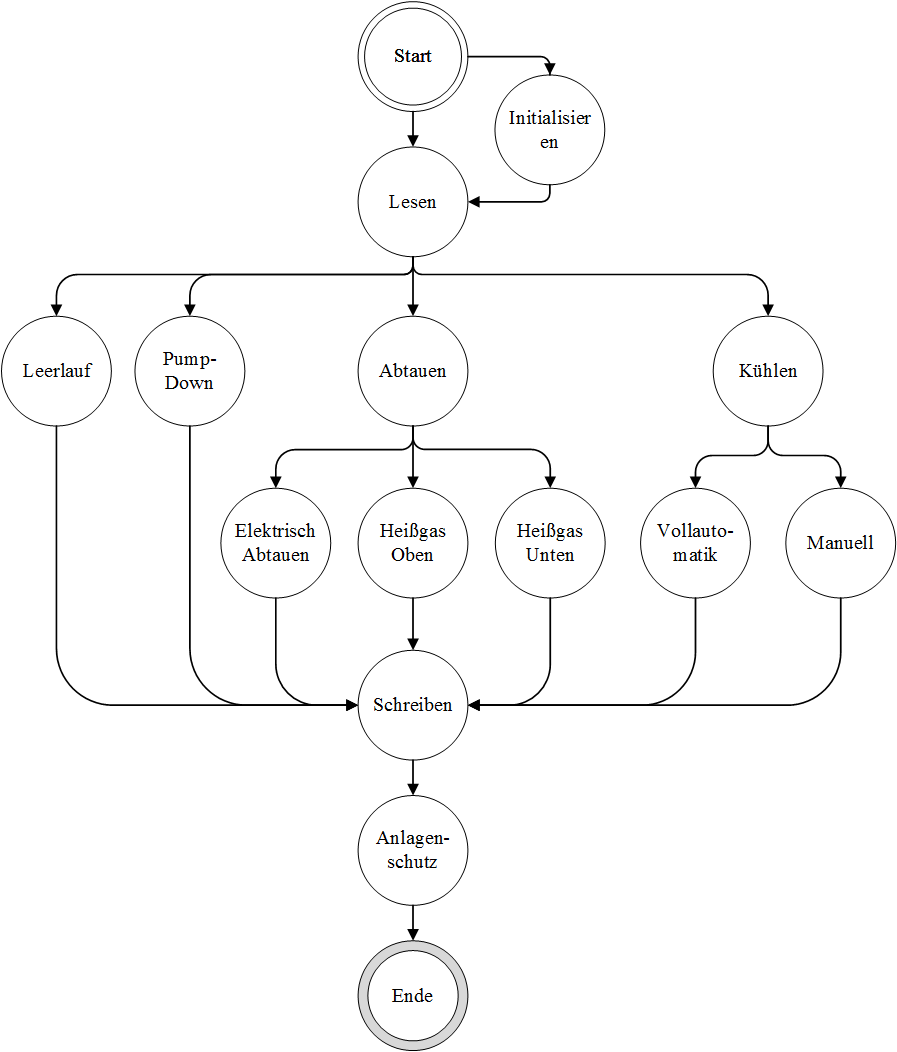
\includegraphics[width=0.90\textwidth]{Pictures/SM.png}
\caption{Status-Maschine}
\label{fig:SM}
\end{figure}

\subsection{Modbus RTU}
\label{subsec:Modbus RTU}

\subsection{Grafical User Interface - GUI}
\label{subsec:GUI}


Drei Hauptzonen sind in der Abbildung farblich dargestellt. Das ist zum einen in \textit{grün} die Kompressor-Einheit. In der \textit{orange} Zone befinden sich der Verflüssiger und der Abtau-Verdampfer. Die \textit{blaue} Zone ist der Verdampfer, er befindet sich innerhalb der KK. Alle Komponenten außerhalb der blauen Zone sind außerhalb der KK installiert. 

 Im Kältekreislauf sind drei Wärmeübertrager installiert: In der \textit{organgenen} Zone sind zwei Wärmeübertrager dargestellt:

\subsection{Anlagenschutz}
\label{subsec: Anlagenschutz}


\chapter{Inbetriebnahme}
\label{cha:Inbetriebnahme}


\section{Kälteanlage}
\label{sec:Inbetriebnahme_KA}


\section{Kalibrierung: Wägesystem}
\label{sec:Kalibrierung Wägesystem}
%%%%%%%%%%%%%%%%%%%%%%%%%%%%%%%%%%%%%%%%%%%%%%%%%%%%%%%%%%%%%%%%%%%%%%%%%%%%%%%

%%%%%%%%%%%%%%%%%%%%%%%%%%%%%%%%%%%%%%%%%%%%%%%%%%%%%%%%%%%%%%%%%%%%%%%%%%%%%%%
% Einbinden der Bibliographie
% Das benötigte File liegt auf dem SVN-Server im Repository
% Nach Möglichkeit bitte dieses File verwenden, da es
% Mehrarbeit erspart!
%%%%%%%%%%%%%%%%%%%%%%%%%%%%%%%%%%%%%%%%%%%%%%%%%%%%%%%%%%%%%%%%%%%%%%%%%%%%%%%
\clearpage
\refstepcounter{Hilfszaehler}
\addcontentsline{toc}{chapter}{\bibname}
\protect\bibliographystyle{natdin}
\bibliography{Literatur}
%%%%%%%%%%%%%%%%%%%%%%%%%%%%%%%%%%%%%%%%%%%%%%%%%%%%%%%%%%%%%%%%%%%%%%%%%%%%%%%


%%%%%%%%%%%%%%%%%%%%%%%%%%%%%%%%%%%%%%%%%%%%%%%%%%%%%%%%%%%%%%%%%%%%%%%%%%%%%%%
% Einbinden des Anhangs
%%%%%%%%%%%%%%%%%%%%%%%%%%%%%%%%%%%%%%%%%%%%%%%%%%%%%%%%%%%%%%%%%%%%%%%%%%%%%%%
\pagestyle{empty}
\clearpage
\vfill{}\vspace{-1\parskip}
\begin{center}\textsf{\textbf{\huge Anhang}}\end{center}{\huge \par}
\vfill{}
\appendix
\newpage
\pagestyle{fancy}
\chapter{Wichtiger Anhang 1}
Weit hinten, hinter den Wortbergen, fern der Länder Vokalien und Konsonantien leben die Blindtexte. Abgeschieden wohnen Sie in Buchstabhausen an der Küste des Semantik, eines großen Sprachozeans. Ein kleines Bächlein namens Duden fließt durch ihren Ort und versorgt sie mit den nötigen Regelialien. Es ist ein paradiesmatisches Land, in dem einem gebratene Satzteile in den Mund fliegen. Nicht einmal von der allmächtigen Interpunktion werden die Blindtexte beherrscht – ein geradezu unorthographisches Leben. Eines Tages aber beschloß eine kleine Zeile Blindtext, ihr Name war Lorem Ipsum, hinaus zu gehen in die weite Grammatik. Der große Oxmox riet ihr davon ab, da es dort wimmele von bösen Kommata, wilden Fragezeichen und hinterhältigen Semikoli, doch das Blindtextchen ließ sich nicht beirren.

\section{Die Versalien}
Es packte seine sieben Versalien, schob sich sein Initial in den Gürtel und machte sich auf den Weg. Als es die ersten Hügel des Kursivgebirges erklommen hatte, warf es einen letzten Blick zurück auf die Skyline seiner Heimatstadt Buchstabhausen, die Headline von Alphabetdorf und die Subline seiner eigenen Straße, der Zeilengasse. Wehmütig lief ihm eine rhetorische Frage über die Wange, dann setzte es seinen Weg fort. Unterwegs traf es eine Copy. Die Copy warnte das Blindtextchen, da, wo sie herkäme wäre sie zigmal umgeschrieben worden und alles, was von ihrem Ursprung noch übrig wäre, sei das Wort "und" und das Blindtextchen solle umkehren und wieder in sein eigenes, sicheres Land zurückkehren. Doch alles Gutzureden konnte es nicht überzeugen und so dauerte es nicht lange, bis ihm ein paar heimtückische Werbetexter auflauerten, es mit Longe und Parole betrunken machten und es dann in ihre Agentur schleppten, wo sie es für ihre Projekte wieder und wieder mißbrauchten.

Und wenn es nicht umgeschrieben wurde, dann benutzen Sie es immernoch. Weit hinten, hinter den Wortbergen, fern der Länder Vokalien und Konsonantien leben die Blindtexte. Abgeschieden wohnen Sie in Buchstabhausen an der Küste des Semantik, eines großen Sprachozeans. Ein kleines Bächlein namens Duden fließt durch ihren Ort und versorgt sie mit den nötigen Regelialien. Es ist ein paradiesmatisches Land, in dem einem gebratene Satzteile in den Mund fliegen. Nicht einmal von der allmächtigen Interpunktion werden die Blindtexte beherrscht – ein geradezu unorthographisches Leben. Eines Tages aber beschloß eine kleine Zeile Blindtext, ihr Name war Lorem Ipsum, hinaus zu gehen in die weite Grammatik. Der große Oxmox riet ihr davon ab, da es dort wimmele von bösen Kommata, wilden Fragezeichen und hinterhältigen Semikoli, doch das Blindtextchen ließ sich nicht beirren. Es packte seine sieben Versalien, schob sich sein Initial in den Gürtel und machte sich auf den Weg. Als es die ersten Hügel des Kursivgebirges erklommen hatte, warf es einen letzten Blick zurück auf die Skyline seiner Heimatstadt Buchstabhausen, die Headline von Alphabetdorf und die Subline seiner eigenen Straße, der Zeilengasse. Wehmütig lief ihm eine rhetorische Frage über die Wange, dann setzte es seinen Weg fort. Unterwegs traf es eine Copy. Die Copy warnte das Blindtextchen, da, wo sie herkäme wäre sie zigmal umgeschrieben worden und alles, was von ihrem Ursprung noch übrig wäre, sei das Wort "und" 

\chapter{Ähnlich wichtiger Anhang}
Es gibt im Moment in diese Mannschaft, oh, einige Spieler vergessen ihnen Profi was sie sind. Ich lese nicht sehr viele Zeitungen, aber ich habe gehört viele Situationen. Erstens: wir haben nicht offensiv gespielt. Es gibt keine deutsche Mannschaft spielt offensiv und die Name offensiv wie Bayern. Letzte Spiel hatten wir in Platz drei Spitzen: Elber, Jancka und dann Zickler. Wir müssen nicht vergessen Zickler. Zickler ist eine Spitzen mehr, Mehmet eh mehr Basler. Ist klar diese Wörter, ist möglich verstehen, was ich hab gesagt? Danke. Offensiv, offensiv ist wie machen wir in Platz. Zweitens: ich habe erklärt mit diese zwei Spieler: nach Dortmund brauchen vielleicht Halbzeit Pause. Ich habe auch andere Mannschaften gesehen in Europa nach diese Mittwoch. Ich habe gesehen auch zwei Tage die Training. Ein Trainer ist nicht ein Idiot! Ein Trainer sei sehen was passieren in Platz. In diese Spiel es waren zwei, drei diese Spieler waren schwach wie eine Flasche leer! Haben Sie gesehen Mittwoch, welche Mannschaft hat gespielt Mittwoch? Hat gespielt Mehmet oder gespielt Basler oder hat gespielt Trapattoni? Diese Spieler beklagen mehr als sie spielen! Wissen Sie, warum die Italienmannschaften kaufen nicht diese Spieler? Weil wir haben gesehen viele Male solche Spiel! Haben 
%%%%%%%%%%%%%%%%%%%%%%%%%%%%%%%%%%%%%%%%%%%%%%%%%%%%%%%%%%%%%%%%%%%%%%%%%%%%%%%


%%%%%%%%%%%%%%%%%%%%%%%%%%%%%%%%%%%%%%%%%%%%%%%%%%%%%%%%%%%%%%%%%%%%%%%%%%%%%%%
% Eigenständigkeitserklärung
%%%%%%%%%%%%%%%%%%%%%%%%%%%%%%%%%%%%%%%%%%%%%%%%%%%%%%%%%%%%%%%%%%%%%%%%%%%%%%%
\cleardoublepage
\pagestyle{empty}
\Large
\textsf{\textbf{Eigenständigkeitserklärung}}


\normalsize
\textsf{Hiermit versichere ich, dass ich die vorliegende Arbeit selbstständig und ohne Benutzung anderer als der angegebenen Hilfsmittel angefertigt habe. Alle Stellen, die wörtlich oder sinngemäß übernommen sind, sind als solche kenntlich gemacht. Die Arbeit ist in gleicher oder ähnlicher Form noch nicht als Prüfungsarbeit eingereicht worden. Ich erkläre mich damit einverstanden, dass die vorliegende Arbeit in der Lehrstuhlbibliothek und Datenbank aufbewahrt und für den internen Gebrauch kopiert werden darf.} \newline \newline


\textsf{Aachen, den \today \newline \newline}


\textsf{Name hier bitte einfügen}

%%%%%%%%%%%%%%%%%%%%%%%%%%%%%%%%%%%%%%%%%%%%%%%%%%%%%%%%%%%%%%%%%%%%%%%%%%%%%%%

\end{document}